 %---------------------------------------------------------------------------%
%-                                                                         -%
%-                           LaTeX Template                                -%
%-                                                                         -%
%---------------------------------------------------------------------------%
%- Copyright (C) Huangrui Mo <huangrui.mo@gmail.com>
%- This is free software: you can redistribute it and/or modify it
%- under the terms of the GNU General Public License as published by
%- the Free Software Foundation, either version 3 of the License, or
%- (at your option) any later version.
%---------------------------------------------------------------------------%
%->> Document class declaration
%---------------------------------------------------------------------------%
\documentclass[printcopy]{Style/neuthesis}%
%- Multiple optional arguments:
%- [<singlesided|doublesided|printcopy>]% set one or two sided eprint or print
%- [draftversion]% show draft version information
%- [fontset=<fandol|windows|mac|adobe>]% specify font set to replace automatic detection
%- [scheme=plain]% thesis writing of international students
%- [standard options for ctex book class: draft|paper size|font size|...]%
%---------------------------------------------------------------------------%
%->> Document settings
%---------------------------------------------------------------------------%
\usepackage[bibtex,myhdr,table,list,geometry]{Style/artratex}
% document settings
%- usage: \usepackage[option1,option2,...,optionN]{artratex}
%- Multiple optional arguments:
%- [bibtex|biber]% set bibliography processor and package
%- [geometry]% reconfigure page layout via geometry package
%- [lscape]% provide landscape layout environment
%- [myhdr]% enable header and footer via fancyhdr package
%- [color]% provide color support via xcolor package
%- [background]% enable page background
%- [tikz]% provide complex diagrams via tikz package
%- [table]% provide complex tables via ctable package
%- [list]% provide enhanced list environments for algorithm and coding
%- [math]% enable some extra math packages
\usepackage{Style/artracom}% user defined commands
%\usepackage{graphicx}
%\usepackage{subfigure}
%\usepackage{booktabs} % For formal tables
\usepackage{xcolor}
\usepackage{color}
\usepackage{fancybox}
\usepackage{listings}
% Color
\definecolor{sr-blue}{rgb}{0.19, 0.55, 0.91}
\definecolor{sr-red}{rgb}{0.89, 0.44, 0.48}
\definecolor{sr-green}{rgb}{0.0, 0.66, 0.47}
\definecolor{sr-yellow}{RGB}{250,249, 222}
\definecolor{sr-gray}{RGB}{63,63,63}

\newcommand{\todo}[1]{\textcolor{sr-red}{TODO: #1}}
\newcommand{\api}[1]{\textcolor{sr-green}{#1}}
\newcommand{\apiarg}[2]{\textcolor{sr-green}{#1}\textcolor{sr-gray}{~(#2)}}
\newcommand{\str}[1]{\texttt{#1}}

\newcommand{\forget}[1]{} 
\usepackage{amsmath}
\newtheorem{theorem}{定理}
\newtheorem{lemma}{引理}
\newtheorem{proof}{证明}
\newtheorem{claim}{声明}
\newtheorem{fact}{事实}
\newtheorem{define}{定义}
\floatname{algorithm}{算法} 


%New colors defined below
\definecolor{codegreen}{rgb}{0,0.6,0}
\definecolor{codegray}{rgb}{0.5,0.5,0.5}
\definecolor{codepurple}{rgb}{0.58,0,0.82}
\definecolor{backcolour}{rgb}{0.95,0.95,0.92}

\definecolor{backcolour}{rgb}{0.95,0.95,0.92}
\definecolor{codegreen}{rgb}{0,0.6,0}


%Code listing style named "mystyle"

\lstdefinestyle{mystyle}{
    backgroundcolor=\color{backcolour}, commentstyle=\color{codegreen},
    keywordstyle=\color{magenta},
    numberstyle=\tiny\color{codegray},
    stringstyle=\color{codepurple},
    basicstyle=\ttfamily\footnotesize,
    breakatwhitespace=false,         
    breaklines=true,                 
    captionpos=b,                    
    keepspaces=true,                 
    numbers=left,                    
    numbersep=5pt,                  
    showspaces=false,                
    showstringspaces=false,
    showtabs=false,                  
    tabsize=2
}

\lstset{style=mystyle}

%---------------------------------------------------------------------------%
%->> Document inclusion
%---------------------------------------------------------------------------%
%\includeonly{Tex/Chap_1,...,Tex/Chap_N}% selected files compilation
%---------------------------------------------------------------------------%
%->> Document content
%---------------------------------------------------------------------------%
\def\alltex{}
\begin{document}
% \layout
%-
%-> Frontmatter: title page, abstract, content list, symbol list, preface
%-
\frontmatter% initialize the environment
%% !TEX ROOT = ../Thesis.tex 
%---------------------------------------------------------------------------%
%->> 封面信息及生成
%---------------------------------------------------------------------------%
%-
%-> 中文封面信息
%-
\category{}%分类号
\confidential{}% 密级:只有涉密论文才填写
\UDC{}
\schoollogo% 校徽
% \schooltitle{width=1cm}{neu_title}
\title{共享资源约束的实时调度理论研究及在OpenMP程序中的应用}% 论文中文题目
\author{杜贺}% 论文作者
\advisor{王义~教授}% 指导教师:姓名 专业技术职务 工作单位
\advisorsec{东北大学计算机科学与工程学院}% 指导老师附加信息 或 第二指导老师信息
\degree{博士}% 学位:学士、硕士、博士
\degreetype{工学}% 学位类别:理学、工学、工程、医学等
\major{计算机应用技术}% 二级学科专业名称
\institute{计算机科学与工程学院}% 院系名称

\research{嵌入式系统}% 研究方向
\authorno{1510409}% 学号
\chinesedate{2021~年~4~月}%  封面页脚日期
\submissiondate{2021~年~4~月}% 论文提交日期
\oraldefencedate{2021~年~4~月}% 论文答辩日期
\degreedate{2021~年~4~月}% 学位授予日期
\chairman{}% 答辩委员会主席
%-
%-> 英文封面信息
%-
\englishtitle{Research on Real-time Scheduling with Shared Resource and Application in OpenMP Program}% 论文英文题目
\englishauthor{He Du}% 论文作者
\englishadvisor{Professor Wang Yi}% 指导教师
\englishdegree{Doctor}% 学位:Bachelor, Master, Doctor。封面格式将根据英文学位名称自动切换,请确保拼写准确无误
\englishdegreetype{Natural Science}% 学位类别:Philosophy, Natural Science, Engineering, Economics, Agriculture 等
\englishthesistype{thesis}% 论文类型: thesis, dissertation
\englishuniversity{Northeastern University}
\englishmajor{Computer Application Technology}% 二级学科专业名称
\englishinstitute{School of Computer Science and Engineering}% 院系名称
\englishdate{April 2021}% 毕业日期:春季 April 夏季为June、秋季为September 冬季为December
%-
%-> 生成封面
%-
%\makereviewcover % 生成盲审中文封面
\makeprintcover %生成打印的中文封面
\makechinesetitle % 生成中文内容页
\makeenglishtitle% 生成英文页
%-
%-> 作者声明
%-
\makedeclaration% 生成声明页
% title page, abstract, dedication
%% !TEX ROOT = ../Thesis.tex 
%-
%-> 中文摘要
%-
\chapter{摘\quad 要}\chaptermark{摘\quad 要}% 摘要标题
% \setcounter{page}{1}% 开始页码
% \pagenumbering{Roman}% 页码符号
% 22p / 12p = 1.83
\linespread{1.5}
\zihao{-4}
% \setlength{\baselineskip}{20pt}

实时系统广泛应用于于航空航天、武器装备、汽车、工业控制、机器人、通信、医疗电子等安全关键应用领域。随着信息技术与人类生活的融合不断加深,实时系统已经成为计算机系统的重要发展方向之一。在实时系统中,任务往往需要互斥访问内存、I/O设备、网络端口等共享资源,操作系统需要设计一定的实时锁协议来确保任务互斥访问共享资源。为了满足系统实时性要求,并且充分利用实时系统的资源,需要实时锁协议,调度算法以及相应的可调度性分析技术相结合,对任务系统调度及资源共享问题进行整体性研究。同时,在多核实时系统中,软件必须要突破应用层级粗粒度并行的局限性,深度挖掘任务内部的细粒度并行特征,使得原本无法满足实时约束的应用软件在多核平台安全运行。OpenMP是高性能计算领域中经典的并行编程框架且众多主流多核嵌入式平台开放对OpenMP的支持,为嵌入式实时系统的并行软件设计与分析提供了绝佳的契机。基于这一背景,本文研究了在共享资源约束下的实时调度技术,本文的主要技术贡献可概括如下:

\begin{itemize}
    \item [(1)]研究了单核上有向图实时任务模型中的嵌套访问共享资源问题。开发了实时锁协议,提出了实时锁协议,并结合最早截止期优先调度策略设计了新的实时调度策略——EDF+N-ACP。并且,提出了针对此调度算法的可调度性分析技术。同时,本文推导出了此调度算法的加速因子,可以用于与其它算法的性能比较。由于实时任务有向图模型加上限制条件后可以推广至其他模型,因此本文中的所有结果均可直接应用于那这些更受限制的模型。
    \item [(2)]研究了多处理器上的锁协议及并行实时任务调度问题,研究了自旋锁对共享资源请求的三种服务顺序,无序,先进先出顺序和固定优先级顺序。在三种服务顺序下,本文提出了对共享资源导致的实时任务阻塞时间的分析方法同时分析了任务系统的最坏响应时间。并且,提出了针对并行实时任务的可调度性分析技术。
    \item [(3)]研究了多处理器上静态OpenMP并行程序分析问题,同时分析了一级私有缓存及二级共享缓存。由于在并行程序的循环时,数据访问指令可能在不同的循环迭代中访问相同的内存块,本文提出了将循环迭代作用域与抽象解释技术相结合的数据缓存分析技术。同时增加了OpenMP框架中循环调度语句对缓存行为的影响。并且基于程序分析结果给出了OpenMP程序适用的循环并行化方案。
    \item [(4)]研究了带有自旋锁的OpenMP实时任务调度问题。在OpenMP程序分析的基础上,对OpenMP实时任务进行细粒度对的建模。通过静态分析OpenMP程序,计算出了OpenMP实时任务参数的安全界限。基于程序的资源模型,提出了针对共享资源导致的阻塞时间分析技术。同时,分析了带自旋锁的OpenMP任务的最坏响应时间,提出了针对OpenMP任务的可调度性分析技术。
\end{itemize}

综上,本文研究了实时系统中在共享资源约束下的实时锁协议及实时任务调度问题。同时研究了基于缓存分析的OpenMP程序分析问题,提出了共享资源约束下OpenMP实时任务的调度技术。本文的研究对实时系统的分析与设计及实时系统中并行程序的分析与设计具有一定的参考价值。

\keywords{实时系统;多核处理器;可调度性分析;共享资源;OpenMP;实时锁协议;最坏响应时间分析;缓存分析}% 中文关键词
%-
%-> 英文摘要
%-
\chapter{Abstract}\chaptermark{Abstract}% 摘要标题

Real-time systems are widely used in safety-critical applications such as aerospace, weaponry, automobiles, industrial control, robotics, communications, and medical electronics. As the integration of information technology and human life continues to deepen, real-time systems have become one of the important development directions of computer systems. In a real-time system, tasks often need to mutually exclusive access to shared resources such as memory, I/O devices, and network ports. The operating system needs to design a certain real-time lock protocol to ensure that tasks mutually exclusive access to shared resources. In order to meet the real-time requirements of the system and make full use of the resources of the real-time system, it is necessary to combine the real-time lock protocol, scheduling algorithm, and corresponding schedulability analysis technology to conduct overall research on task system scheduling and resource sharing. At the same time, in a multi-core real-time system, the software must break through the limitations of application-level coarse-grained parallelism, and drill down to the fine-grained parallel features within tasks, so that application software that cannot meet real-time constraints can run safely on a multi-core platform. OpenMP is a classic parallel programming framework in the field of high-performance computing, and many mainstream multi-core embedded platforms open to support OpenMP, providing an excellent opportunity for parallel software design and analysis of embedded real-time systems. Based on this background, this paper studies the real-time scheduling technology under the constraints of shared resources. The main contributions of this paper can be summarized as follows:

\begin{itemize}
    \item [(1)] The problem of nested access to shared resources in the real-time task model of directed graphs on a single core is studied. Developed the real-time lock protocol, proposed the real-time lock protocol, and designed a new real-time scheduling strategy—EDF+N-ACP based on the earliest deadline priority scheduling strategy. In addition, a schedulability analysis technique for this scheduling algorithm is proposed. At the same time, this article deduces the acceleration factor of this scheduling algorithm, which can be used to compare the performance of other algorithms. Since the real-time task directed graph model can be extended to other models with restrictions, all the results in this article can be directly applied to these more restricted models.
    
    \item [(2)] The lock protocol and parallel real-time task scheduling on multi-processors are studied, and the three service orders of spin locks for shared resource requests, disorder, first-in first-out order and fixed priority order are studied. Under the three service sequences, this paper proposes an analysis method for the blocking time of real-time tasks caused by shared resources and analyzes the worst response time of the task system. In addition, a schedulability analysis technique for parallel real-time tasks is proposed.
    
    \item [(3)] The analysis of static OpenMP parallel programs on multi-processors is studied, and the first-level private cache and the second-level shared cache are also analyzed. Because in the loop of a parallel program, data access instructions may access the same memory block in different loop iterations, this paper proposes a data cache analysis technology that combines loop iteration scope with abstract interpretation technology. At the same time, the impact of the circular scheduling statement in the OpenMP framework on the cache behavior is increased. And based on the results of program analysis, a suitable loop parallelization scheme for OpenMP programs is given.
    
    \item [(4)] The OpenMP real-time task scheduling problem with spin lock is studied. On the basis of OpenMP program analysis, the OpenMP real-time task is modeled fine-grained. Through static analysis of the OpenMP program, the safety limits of the OpenMP real-time task parameters are calculated. Based on the resource model of the program, an analysis technique for blocking time caused by shared resources is proposed. At the same time, the worst response time of OpenMP tasks with spin locks is analyzed, and a schedulability analysis technique for OpenMP tasks is proposed.
\end{itemize}

In summary, this dissertation studies the real-time lock protocol and real-time task scheduling under the constraints of shared resources in real-time systems. Meanwhile, the OpenMP program analysis problem based on cache analysis is studied, and the scheduling technology of OpenMP real-time tasks under the constraint of shared resources is proposed. The results of this dissertation serve as theoretical foundations as well as provides insights for design and analysis real-time system and parallel programs.


\englishkeywords{Real-time system; multi-core processor; schedulability analysis; shared resources; OpenMP; real-time locking protocol; worst-case response time analysis; cache analysis}
 % abstract (chinese and english)


{% content list region
% \linespread{1}
% \intotoc{\contentsname}% add link to contents table and bookmark
% \chapter*{\contentsname}
\linespread{1.5}% local line space
\tableofcontents% contents catalog

\forget{
\intotoc{\listfigurename}% add link to contents table and bookmark
\listoffigures% figures catalog

\intotoc{\listtablename}% add link to contents table and bookmark
\listoftables% tables catalog
}

}


% \input{Tex/Prematter}% list of symbols, preface content
%-
%-> Mainmatter
%-
\mainmatter% initialize the environment
\linespread{1.4}
\zihao{-4}
%---------------------------------------------------------------------------%
%->> Main content
%---------------------------------------------------------------------------%


\chapter{Overview of uROS}
\section{Structure of uROS}

\section{Basic Concepts}
The major concepts (publishers, subscriptions, services, timers, ...) are identical with ROS2. They even rely on the same implementation, as the micro-ROS C API is based on the ROS 2 client support library (rcl), enriched with a set of convenience functions by the package rclc\footnote{(https://github.com/ros2/rclc/)}. That is, rclc does not add a new layer of types on top of rcl (like rclcpp and rclpy do) but only provides functions that ease the programming with the rcl types. New types are introduced only for concepts that are missing in rcl, such as the concept of an executor.

% - NOTE:
\subsection{Nodes}
Each node in ROS should be responsible for a single, module purpose (e.g. one node for controlling wheel motors, one node for controlling a laser range-finder, etc). Each node can send and receive data to other nodes via topics, services, actions, or parameters.
\begin{figure}[htb!]
    \centering
    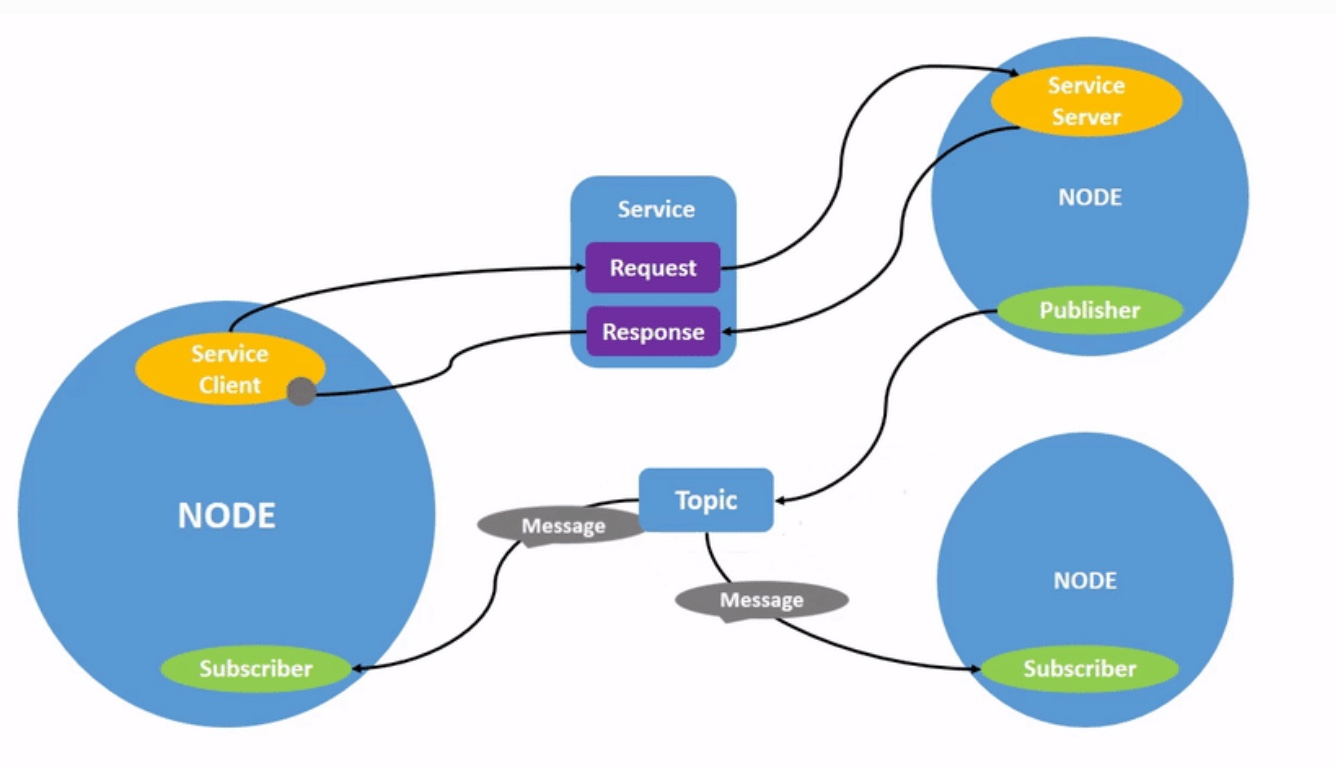
\includegraphics[width=0.75\linewidth]{Img/node.jpg}
    \caption{Nodes}\label{f:node}
    \vspace{-0.1in}
\end{figure}

\subsubsection{Initialization}
\textbf{1. Create a node with default configuration:}
\begin{lstlisting}[language=Python, caption=Python example]
    // Initialize micro-ROS allocator
    rcl_allocator_t allocator = rcl_get_default_allocator();
    
    // Initialize support object
    rclc_support_t support;
    rcl_ret_t rc = rclc_support_init(&support, argc, argv, &allocator);
    
    // Create node object
    rcl_node_t node;
    const char * node_name = "test_node";
    
    // Node namespace (Can remain empty "")
    const char * namespace = "test_namespace";
    
    // Init default node
    rc = rclc_node_init_default(&node, node_name, namespace, &support);
    if (rc != RCL_RET_OK) {
        ... // Handle error
        return -1;
    }
\end{lstlisting}

\textbf{2. Create a node with custom options:} The configuration of the node will also be applied to its future elements (Publishers, subscribers, services, \dots). The API used to customize the node options differs between ROS2 distributions:

Foxy: The \api{rcl\_node\_options\_t} is used to configure the node
\begin{lstlisting}[language=Python, caption=Python example]
// Initialize allocator and support objects
...

// Create node object
rcl_node_t node;
const char * node_name = "test_node";

// Node namespace (Can remain empty "")
const char * namespace = "test_namespace";

// Get default node options and modify them
rcl_node_options_t node_ops = rcl_node_get_default_options();

// Set node ROS domain ID to 10
node_ops.domain_id = (size_t)(10);

// Init node with custom options
rc = rclc_node_init_with_options(&node, node_name, namespace, &support, &node_ops);

if (rc != RCL_RET_OK) {
... // Handle error
return -1;
}
\end{lstlisting}

Galactic: In this case, the node options are configured on the \api{rclc\_support\_t} object with a custom API
\begin{lstlisting}[language=Python, caption=Python example]
// Initialize micro-ROS allocator
rcl_allocator_t allocator = rcl_get_default_allocator();

// Initialize and modify options (Set DOMAIN ID to 10)
rcl_init_options_t init_options = rcl_get_zero_initialized_init_options();
rcl_init_options_init(&init_options, allocator);
rcl_init_options_set_domain_id(&init_options, 10);

// Initialize rclc support object with custom options
rclc_support_t support;
rclc_support_init_with_options(&support, 0, NULL, &init_options, &allocator);

// Create node object
rcl_node_t node;
const char * node_name = "test_node";

// Node namespace (Can remain empty "")
const char * namespace = "test_namespace";

// Init node with configured support object
rclc_node_init_default(&node, node_name, namespace, &support);

if (rc != RCL_RET_OK) {
... // Handle error
return -1;
}
\end{lstlisting}

\textbf{3. Cleaning up:} To destroy a initialized node all entities owned by the node (Publishers, subscribers, services, \dots) have to be destroyed before the node itself. This will delete the node from ROS2 graph, including any generated infrastructure on the agent (if possible) and used memory on the client.
\begin{lstlisting}[language=Python, caption=Python example]
// Destroy created entities (Example)
rcl_publisher_fini(&publisher, &node);
...

// Destroy the node
rcl_node_fini(&node);
\end{lstlisting}

% - NOTE: 
\subsection{Publishers and subscribers}
ROS 2 publishers and subscribers are the basic communication mechanism between nodes using topics. Ready to use code related to this concepts can be found in \href{https://github.com/micro-ROS/micro-ROS-demos/blob/foxy/rclc/int32_publisher/main.c}{micro-ROS-demos/rclc/int32\_publisher} and \href{https://github.com/micro-ROS/micro-ROS-demos/blob/foxy/rclc/int32_subscriber/main.c}{micro-ROS-demos/rclc/int32\_subscriber} folders. Fragments of code from this examples are used on this tutorial. ROS 2 breaks complex systems down into many modular nodes. Topics are a vital element of the ROS graph that act as a bus for nodes to exchange messages.
\begin{figure}[htb!]
    \centering
    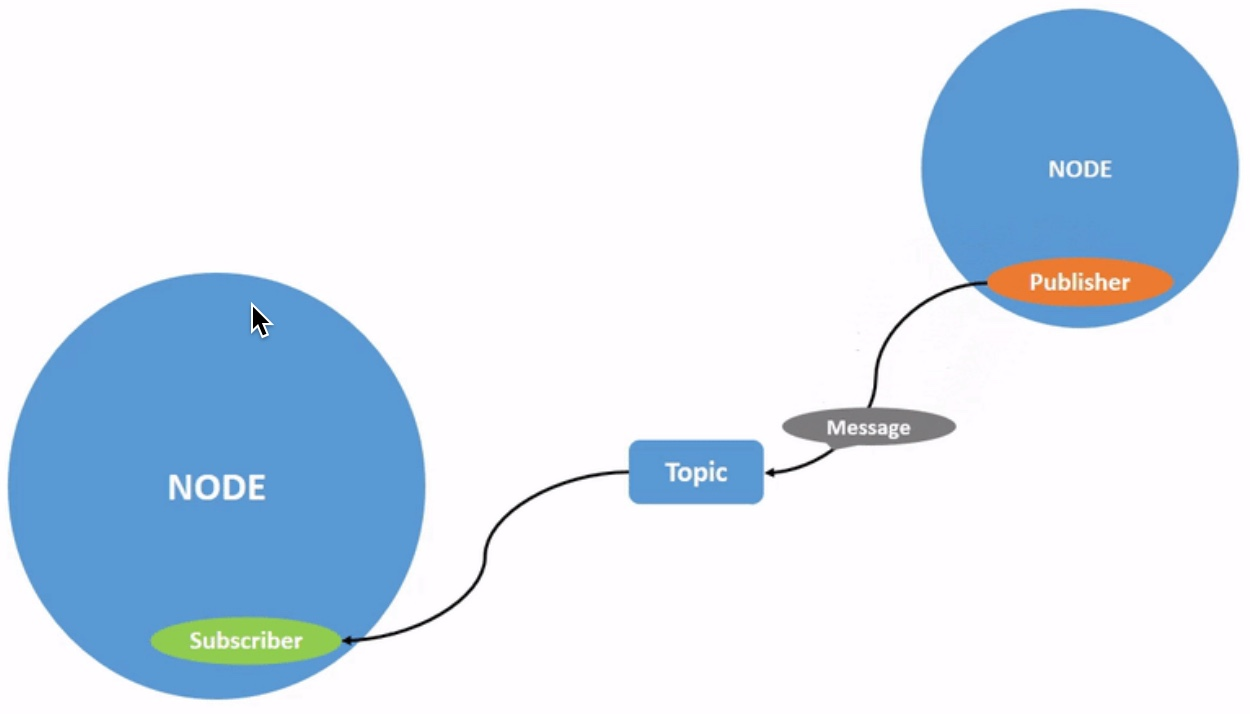
\includegraphics[width=0.55\linewidth]{Img/topic.jpg}
    \caption{Publishers and subscribers}\label{f:topic}
    \vspace{-0.1in}
\end{figure}

A node may publish data to any number of topics and simultaneously have subscriptions to any number of topics. Topics are one of the main ways in which data is moved between nodes and therefore between different parts of the system.
\begin{figure}[htb!]
    \centering
    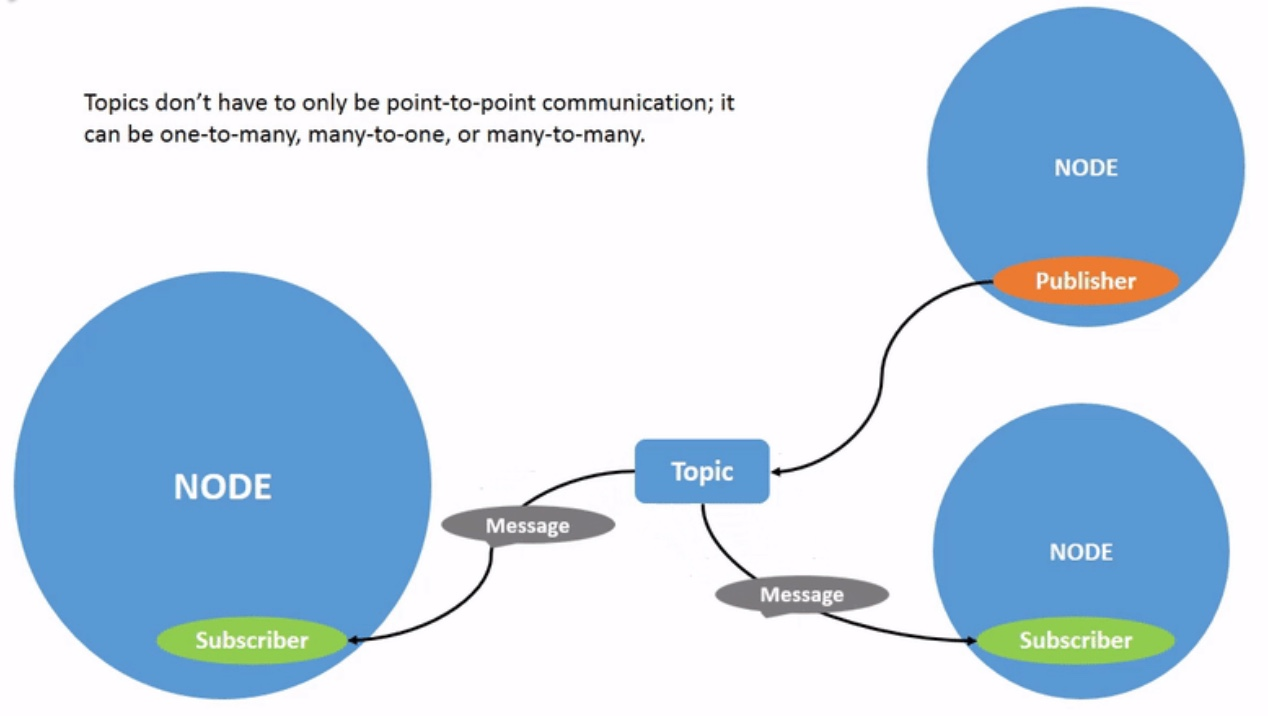
\includegraphics[width=0.55\linewidth]{Img/topic2.jpg}
    \caption{Publishers and subscribers}\label{f:topic2}
    \vspace{-0.1in}
\end{figure}

\subsubsection{Publisher}
\textbf{1. Initialization:} Starting from a code where RCL is initialized and a micro-ROS node is created, there are tree ways to initialize a publisher depending on the desired quality-of-service configuration. For a detail on the available QoS options and the advantages and disadvantages between reliable and best effort modes, check the \href{https://micro.ros.org/docs/tutorials/programming_rcl_rclc/qos/}{QoS tutorial}.

\begin{lstlisting}[language=Python, caption=Reliable (default)]
    // Publisher object
    rcl_publisher_t publisher;
    const char * topic_name = "test_topic";
    
    // Get message type support
    const rosidl_message_type_support_t * type_support =
        ROSIDL_GET_MSG_TYPE_SUPPORT(std_msgs, msg, Int32);
    
    // Creates a reliable rcl publisher
    rcl_ret_t rc = rclc_publisher_init_default(
        &publisher, &node,
        &type_support, &topic_name);
    
    if (RCL_RET_OK != rc) {
        ...  // Handle error
        return -1;
    }
\end{lstlisting}

\begin{lstlisting}[language=Python, caption=Best effort]
    // Publisher object
    rcl_publisher_t publisher;
    const char * topic_name = "test_topic";
    
    // Get message type support
    const rosidl_message_type_support_t * type_support =
        ROSIDL_GET_MSG_TYPE_SUPPORT(std_msgs, msg, Int32);
    
    // Creates a best effort rcl publisher
    rcl_ret_t rc = rclc_publisher_init_best_effort(
        &publisher, &node,
        &type_support, &topic_name);
    
    if (RCL_RET_OK != rc) {
        ...  // Handle error
        return -1;
    }
\end{lstlisting}

\begin{lstlisting}[language=Python, caption=Custom QoS]
    // Publisher object
    rcl_publisher_t publisher;
    const char * topic_name = "test_topic";
    
    // Get message type support
    const rosidl_message_type_support_t * type_support =
        ROSIDL_GET_MSG_TYPE_SUPPORT(std_msgs, msg, Int32);
    
    // Set publisher QoS
    const rmw_qos_profile_t * qos_profile = &rmw_qos_profile_default;
    
    // Creates a rcl publisher with customized quality-of-service options
    rcl_ret_t rc = rclc_publisher_init(
        &publisher, &node,
        &type_support, &topic_name, qos_profile);
    
    if (RCL_RET_OK != rc) {
        ...  // Handle error
        return -1;
    }
\end{lstlisting}

\textbf{2. Publish a message:} Use \api{rcl\_publish} to publish messages to the topic. For periodic publications, \api{rcl\_publish}\footnote{Note that \api{rcl\_publish} is thread safe and can be called from multiple threads.} can be placed inside a timer callback. Check the \href{https://micro.ros.org/docs/tutorials/programming_rcl_rclc/executor/}{Executor and timers section} for details.

\begin{lstlisting}[language=Python, caption=publish messages]
    // Int32 message object
    std_msgs__msg__Int32 msg;
    
    // Set message value
    msg.data = 0;
    
    // Publish message
    rcl_ret_t rc = rcl_publish(&publisher, &msg, NULL);
    
    if (rc != RCL_RET_OK) {
        ...  // Handle error
        return -1;
    }
\end{lstlisting}


\subsubsection{Subscriber}
\textbf{1. Initialization:} The subscription initialization is almost identical to the publisher one:

\begin{lstlisting}[language=Python, caption=Reliable (default)]
    // Subscription object
    rcl_subscription_t subscriber;
    const char * topic_name = "test_topic";
    
    // Get message type support
    const rosidl_message_type_support_t * type_support =
        ROSIDL_GET_MSG_TYPE_SUPPORT(std_msgs, msg, Int32);
    
    // Initialize a reliable subscriber
    rcl_ret_t rc = rclc_subscription_init_default(
        &subscriber, &node,
        &type_support, &topic_name);
    
    if (RCL_RET_OK != rc) {
        ...  // Handle error
        return -1;
    }
\end{lstlisting}

\begin{lstlisting}[language=Python, caption=Best effort]
    // Subscription object
    rcl_subscription_t subscriber;
    const char * topic_name = "test_topic";
    
    // Get message type support
    const rosidl_message_type_support_t * type_support =
        ROSIDL_GET_MSG_TYPE_SUPPORT(std_msgs, msg, Int32);
    
    // Initialize best effort subscriber
    rcl_ret_t rc = rclc_subscription_init_best_effort(
        &subscriber, &node,
        &type_support, &topic_name);
    
    if (RCL_RET_OK != rc) {
        ...  // Handle error
        return -1;
    }
\end{lstlisting}

\begin{lstlisting}[language=Python, caption=Custom QoS]
    // Subscription object
    rcl_subscription_t subscriber;
    const char * topic_name = "test_topic";
    
    // Get message type support
    const rosidl_message_type_support_t * type_support =
        ROSIDL_GET_MSG_TYPE_SUPPORT(std_msgs, msg, Int32);
    
    // Set client QoS
    const rmw_qos_profile_t * qos_profile = &rmw_qos_profile_default;
    
    // Initialize a subscriber with customized quality-of-service options
    rcl_ret_t rc = rclc_subscription_init(
        &subscriber, &node,
        &type_support, &topic_name, qos_profile);
    
    if (RCL_RET_OK != rc) {
        ...  // Handle error
        return -1;
    }
\end{lstlisting}

\textbf{2. Callbacks:} The executor is responsible to call the configured callback when a message is published. The function will have the message as its only argument, containing the values sent by the publisher:
\begin{lstlisting}[language=Python, caption=Sub-callback decalaration]
    // Function prototype:
    void (* rclc_subscription_callback_t)(const void *);
    
    // Implementation example:
    void subscription_callback(const void * msgin)
    {
        // Cast received message to used type
        const std_msgs__msg__Int32 * msg = (const std_msgs__msg__Int32 *)msgin;
    
        // Process message
        printf("Received: %d\n", msg->data);
    }
\end{lstlisting}

Once the subscriber and the executor are initialized, the subscriber callback must be added to the executor to receive incoming publications once its spinning:
\begin{lstlisting}[language=Python, caption=Sub-callback registration]
    // Message object to receive publisher data
    std_msgs__msg__Int32 msg;
    
    // Add subscription to the executor
    rcl_ret_t rc = rclc_executor_add_subscription(
        &executor, &subscriber, &msg,
        &subscription_callback, ON_NEW_DATA);
    
    if (RCL_RET_OK != rc) {
        ...  // Handle error
        return -1;
    }
    
    // Spin executor to receive messages
    rclc_executor_spin(&executor);
\end{lstlisting}

\subsubsection{Message initialization}
Before publishing or receiving a message, it may be necessary to initialize its memory for types with strings or sequences. Check the \href{https://micro.ros.org/docs/tutorials/advanced/handling_type_memory/}{Handling messages memory in micro-ROS} section for details.

\subsubsection{Cleaning Up}
After finishing the publisher/subscriber, the node will no longer be advertising that it is publishing/listening on the topic. To destroy an initialized publisher or subscriber:
\begin{lstlisting}[language=Python, caption=To destroy an initialized publisher or subscriber]
// Destroy publisher
rcl_publisher_fini(&publisher, &node);

// Destroy subscriber
rcl_subscription_fini(&subscriber, &node);
\end{lstlisting}





% - NOTE: Services
\subsection{Services}
Services are another method of communication for nodes in the ROS graph. Services are based on a call-and-response model, versus topics’ publisher-subscriber model. While topics allow nodes to subscribe to data streams and get continual updates, services only provide data when they are specifically called by a client. Ready to use code related to this concepts can be found in \href{https://github.com/micro-ROS/micro-ROS-demos/blob/foxy/rclc/addtwoints_server/main.c}{micro-ROS-demos/rclc/addtwoints\_server} and \href{https://github.com/micro-ROS/micro-ROS-demos/blob/foxy/rclc/addtwoints_client/main.c}{micro-ROS-demos/rclc/addtwoints\_client} folders. Fragments of code from this examples are used on this tutorial.
\begin{figure}[htb!]
    \centering
    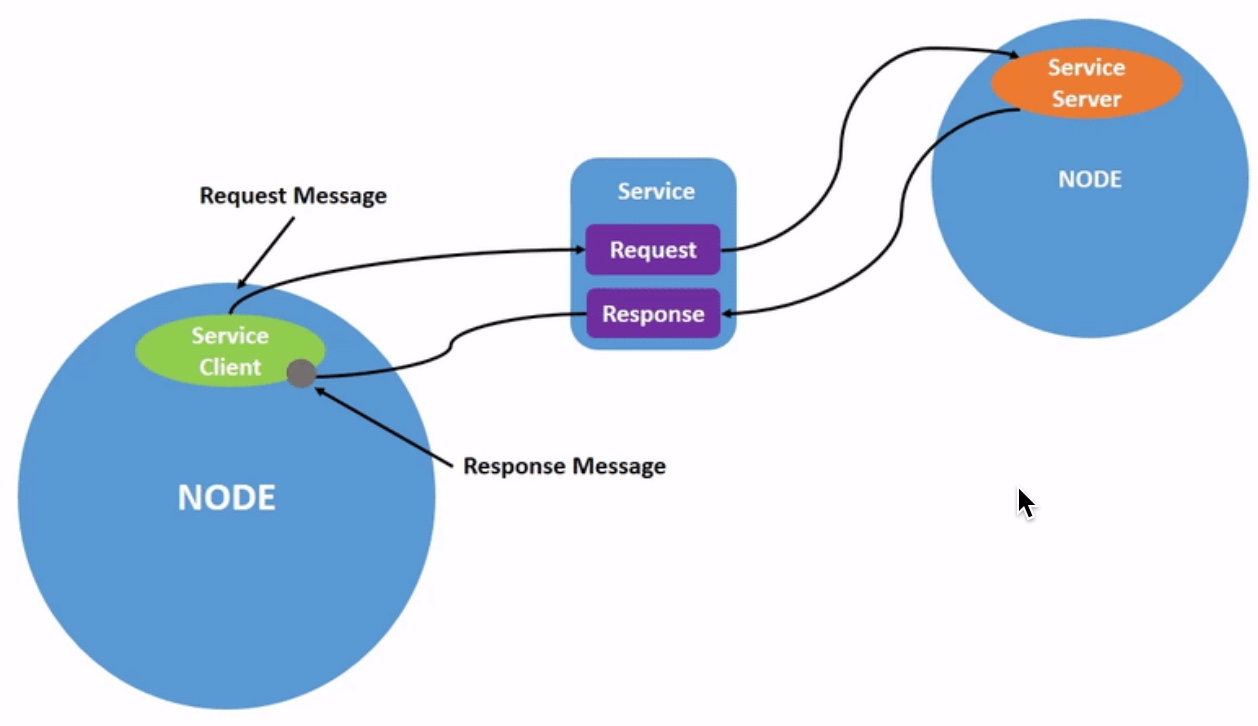
\includegraphics[width=0.75\linewidth]{Img/service1.jpg}
    \caption{Service}
    \vspace{-0.1in}
\end{figure}
\begin{figure}[htb!]
    \centering
    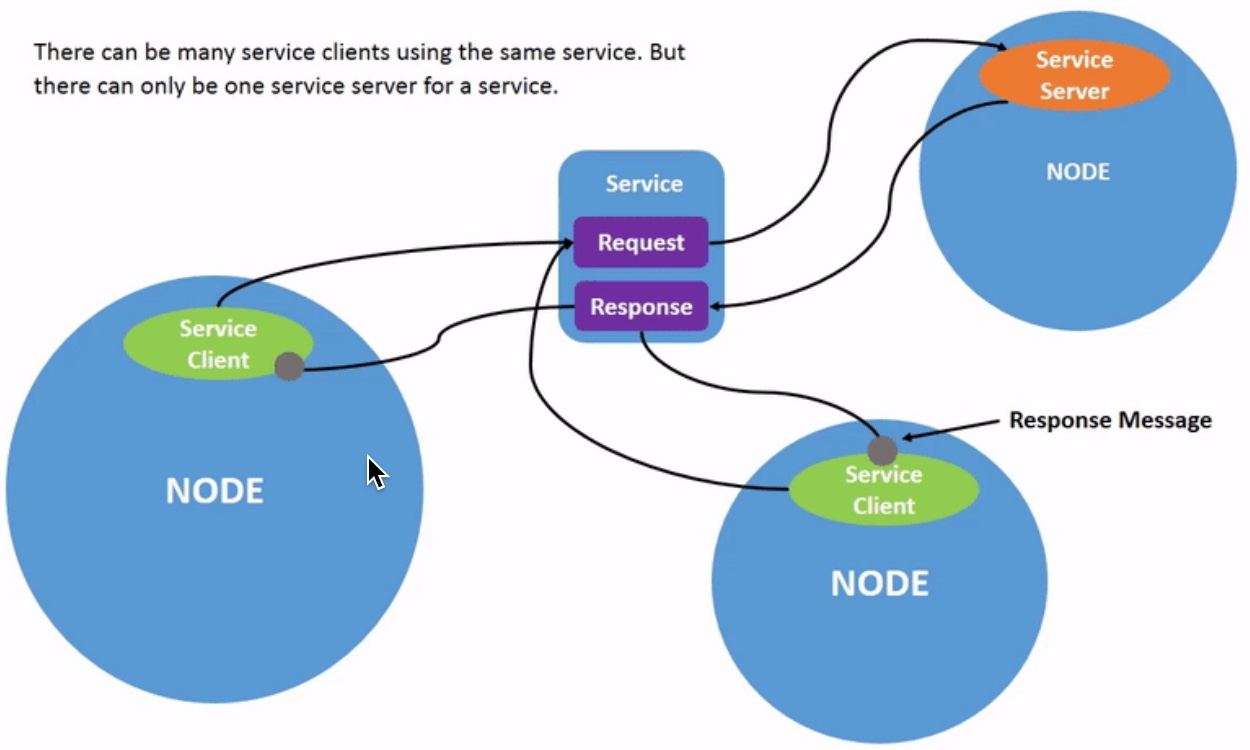
\includegraphics[width=0.75\linewidth]{Img/service2.jpg}
    \caption{Service2}
    \vspace{-0.1in}
\end{figure}

\todo{https://micro.ros.org/docs/tutorials/programming\_rcl\_rclc/service/}
\subsubsection{Service server}
\subsubsection{Service Client}
\subsubsection{Message initialization}
\subsubsection{Cleaning Up}


\subsection{Parameter server}
\todo{https://micro.ros.org/docs/tutorials/programming\_rcl\_rclc/parameters/}

\subsection{Executor and timers}
\subsubsection{Timer}
Timers can be created and added to the executor, which will call the timer callback periodically once it is spinning. They are usually used to handle periodic publications or events.

\textbf{1. Initialization:}
\begin{lstlisting}[language=Python, caption=Timer Initialization]
    // Timer period on nanoseconds
    const unsigned int timer_period = RCL_MS_TO_NS(1000);
    // Create and initialize timer object
    rcl_timer_t timer;
    rcl_ret_t rc = rclc_timer_init_default(&timer, &support, timer_period, timer_callback);
    // Add to the executor
    rc = rclc_executor_add_timer(&executor, &timer);
    if (rc != RCL_RET_OK) {
        ... // Handle error
        return -1;
    }    
\end{lstlisting}

\textbf{2. Callback:} The callback gives a pointer to the associated timer and the time elapsed since the previous call or since the timer was created if it is the first call to the callback. During the callback the timer can be canceled or have its period and/or callback modified using the passed pointer. Check rcl/timer.h for details.
\begin{lstlisting}[language=Python, caption=Timer Callback]
    void timer_callback(rcl_timer_t * timer, int64_t last_call_time)
    {
        printf("Last callback time: %ld\n", last_call_time);
    
        if (timer != NULL) {
            // Perform actions
            ...
        }
    }  
\end{lstlisting}

\textbf{3. Cleaning Up:} To destroy an initialized timer, This will deallocate used memory and make the timer invalid.
\begin{lstlisting}[language=Python, caption=Timer Cleaning up]
    // Destroy timer
    rcl_timer_fini(&timer);
    This will deallocate used memory and make the timer invalid    
\end{lstlisting}



\subsubsection{Executor}

\subsection{Quality of service}

\subsection{micro-ROS utilities}

\section{Data Distribution Service (DDS)}
\textbf{DDS itself is an API specification and the actual underlying protocol is the Real-Time Publish-Subscribe Protocol (RTPS)\cite{RTPS}.} Multiple open-source implementations of DDS are available for full-fledged computers running Linux or Windows. Few implementations are suitable for resource-constrained embedded systems.

eProsima FastRTPS is a popular RTPS implementation that is also the underlying middleware for ROS 2. OpenDDS is another widespread implementation that is a DDS implementation on top of the RTPS protocol~\cite{OpenDDS}. Real-Time Innovations (RTI) offers ConnextDDS, a commercial DDS implementation~\cite{ConnextDDS}. All of the implementations mentioned above target Linux, Windows or MacOS and do not run on embedded platforms. RTI also offers microDDS, an implementation suitable for microcontrollers. In contrast to embeddedRTPS~\cite{kampmann2019portable}, microDDS is not open source and only commercially available. Lastly, freeRTPS 2 is an implementation originally developed for microcontrollers in the context of ROS 2. This implementation explicitly targets STM32 microprocessors and is not under active maintenance.

The DDS Extremely Resource Constrained Environments (XRCE) standard is intended for integration of embedded systems into DDS networks~\cite{XRCE}. The resource-constrained platform is integrated into the DDS network by a more powerful server, that acts as a gateway. \textbf{In this architecture, the microcontroller is not an independent, first-class participant in the communication network, as it's ability to communicate depends on server.} This also introduces a single point of failure, rendering this architecture potentially unsuitable for safety-critical applications.

\subsection{Background of RTPS}
This section provides a brief overview of the basic concepts behind RTPS. We cover the basic entities, the discovery procedure and data exchange mechanisms. An exhaustive description is provided in the standard maintained by the OMG~\cite{RTPS}.

\subsubsection{Entities}
As depicted in Fig. \ref{f:rtps}, the basic actors in RTPS are \textit{participants}, which in turn have a variable number of readers or writers. Readers or writers (summarized as \textit{endpoints} in the following) can be identified with an id composed of a unique participant prefix and an entity id which is unique within this participant. They communicate through a publish-subscribe mechanism, a concept also common in other messaging frameworks such as ROS or Message Queuing Telemetry Transport (MQTT). \textbf{Endpoints are loosely coupled only by a topic name and data type definition.} From a user perspective, messages published by writers are addressed to a topic and not to specific recipients. Respectively, readers subscribe to a specific topic and join the network without knowledge about the specific writer(s). For this, participants become aware of each other during runtime in the course of a decentralized discovery process. Thus, readers and writers form a loosely coupled communication network that is suitable for runtime integrated systems.
\begin{figure}[htb!]
    \centering
    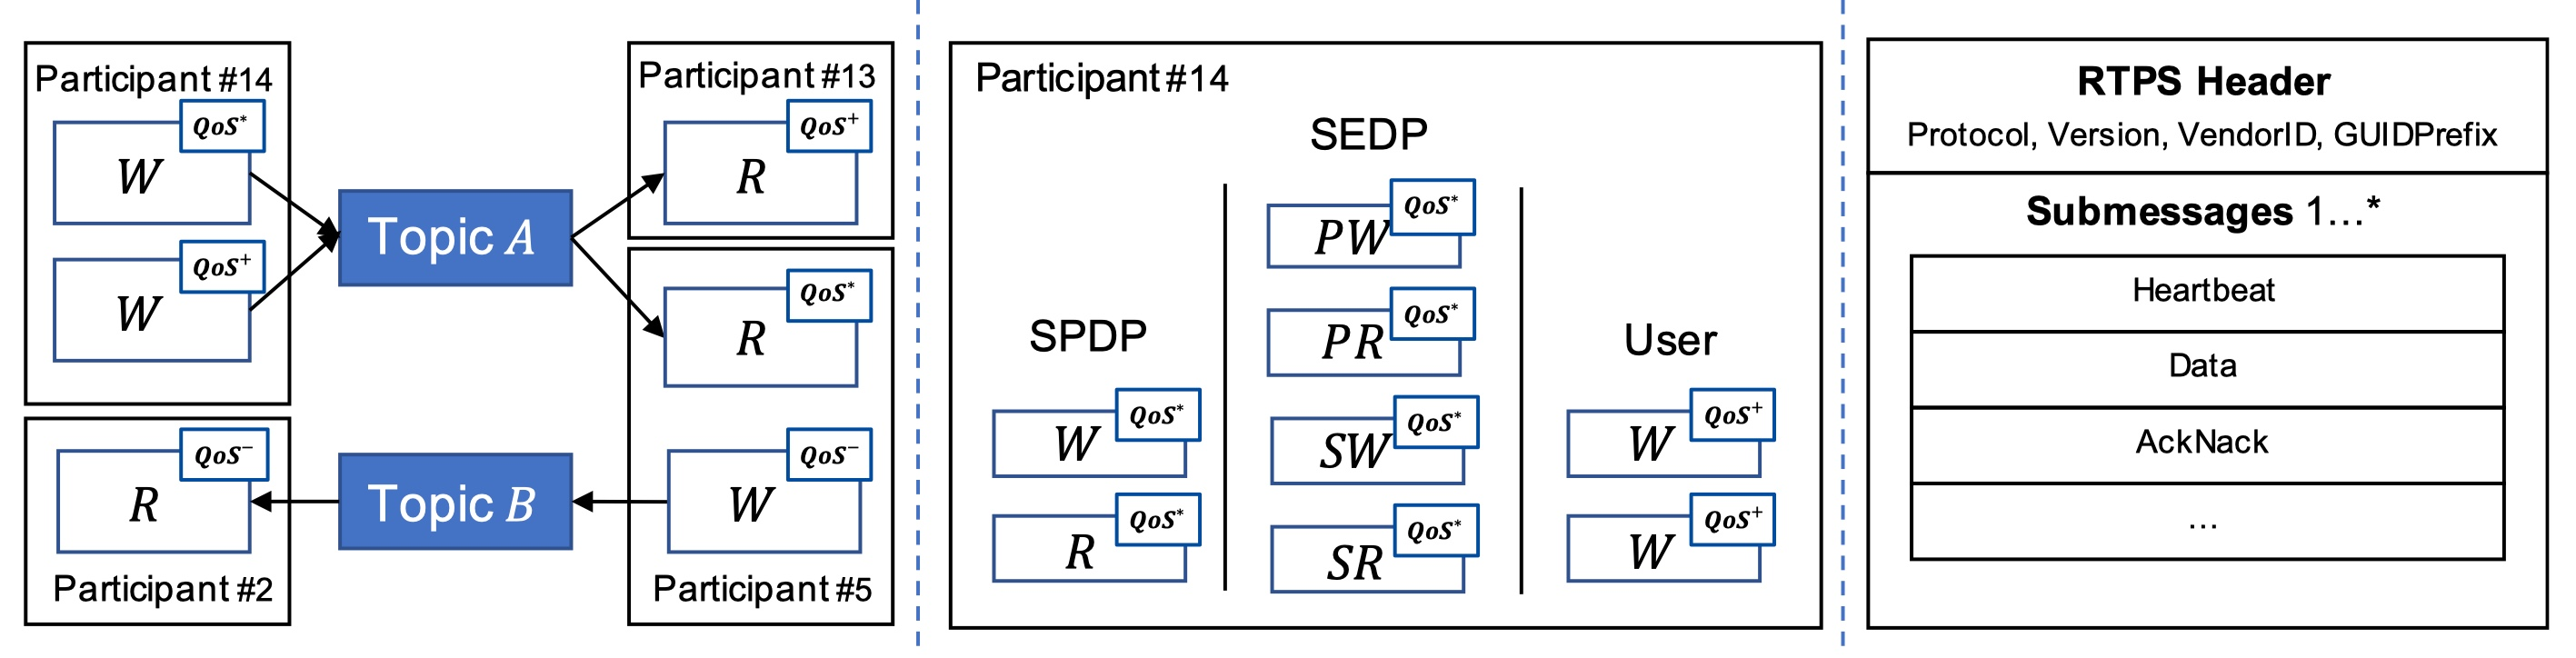
\includegraphics[width=0.95\linewidth]{Img/RTPS.jpg}
    \caption{\text{Left}: Participants Exchange Messages via User-defined Reader and Writer Endpoints. \textbf{Middle}: Built-in RTPS endpoints for Participant (SPDP) and Endpoint Discovery (SEDP) alongside user-defined Endpoints. \textbf{Right}: Components of RTPS Messages encapsulated in UDP Packets.}\label{f:rtps}
    \vspace{-0.1in}
\end{figure}

Various Quality of Service (QoS) parameters can be used to customize the behavior of endpoints. For example, writers and readers communicate either in a \textit{reliable} or \textit{best-effort} mode. \textbf{Reliable writers keep track of already transmitted packages through sequence numbers and are able to resend messages in case of a transmission failure. Best-effort writers do not provide this capability.} The user interacts with endpoints by passing serialized data to writers or receiving data from readers. RTPS is specified for TCP/UDP communication.

In general, endpoints send \underline{UDP packets} that are structured as depicted in Fig. \ref{f:rtps}. Each message starts with a header that contains, among other fields, the RTPS version or vendor identification. The header is followed by a variable amount of sub-messages that are used for data exchange and discovery. \texttt{Data} sub-messages are used to exchange generic, serialized data between readers and writers. \texttt{Heartbeat} and \texttt{AckNack} sub-messages are used to provide a reliable communication. The \texttt{Heartbeat} sub-message allows writers to announce the available sequence numbers in its storage. Reliable readers send \texttt{AckNack} sub-messages to communicate missing as well as received packets. Based on those acknowledgments, the reliable writer can decide when a packet can be safely removed from its history. While one or multiple participants are addressed by a specific port, the target endpoint is identified by the entity id passed with the aforementioned messages.

\subsubsection{Discovery Protocols}
Entities in RTPS discover each other through a decentralized two-step discovery process, using a set of six built-in endpoints as depicted in Fig. \ref{f:rtps}. Technically, these are regular endpoints that function just like user-defined endpoints but communicate specific messages for the discovery process and have a fixed entity id. In the first step, the Simple Participant Discovery Protocol (SPDP) uses a reader/writer pair of best-effort endpoints for discovery of participants and their properties in the network. Each participant periodically sends messages through the SPDP-writer containing information about the participant on standardized IP broadcast addresses. The transmitted UDP packets are made up of RTPS packets containing a \texttt{Data} sub-message and are received by remote SPDP-readers. Discovery of those endpoints is not required because the messages are send on addresses which are relevant for all participants and the destination is known as the built-in endpoints have fixed entity ids. SPDP messages contain, among others, the unicast or multicast locators (i.e. IP-address and port) for meta (e.g. discovery) and user traffic to the sending participant.

Once the participants become aware of each other, they exchange information about user-defined endpoints using the Simple Endpoint Discovery Protocol (SEDP). For this, reliable writers and readers are used. The publication writer PW sends information about user-defined writers to all known participants by addressing the publication readers PR of all known participants. For each user-defined endpoint, information about it’s QoS parameters, locators and their entity id are transmitted. Analogously, user-defined readers are announced through the subscription-writer SW and participants receive these respective messages through the subscription-reader SR. After discovering a new endpoint, a participant tries to match it with one if its own endpoints. Endpoints are matched if the topic name, data type name and QoS parameters are compatible.

Once local endpoints have been matched with remote endpoints, every message that is handed to the writer will be send to all known, matching readers in the network. For this purpose, the user hands over a serialized byte array, that is inserted into RTPS packet containing a \texttt{Data} sub-message. Note that SPDP and SEDP messages are sent periodically, therefore participants and endpoints can dynamically join the RTPS network.
\chapter{Design of uROS}
\section{RCLC}
\subsection{RCLC-Executor}
Here we introduce the rclc Executor, which is a ROS 2 Executor implemented based on and for the rcl API, for applications written in the C language. Often embedded applications require real-time to guarantee end-to-end latencies and need deterministic runtime behavior to correctly replay test data. However, this is difficult with the default ROS 2 Executor because of its complex semantics, as discussed in the previous section.

First, we will analyse the requirements for real-time embedded applications and, secondly, derive simple features for an Executor to enable deterministic and real-time behavior. Then we will present the API of the RCLC-Executor and provide example usages of the RCLC-Executor to address these requirements.

\subsubsection{Requirement Analysis}
\todo{Real-time embedded application use-case and LET\footnote{https://github.com/ros2/rclc/tree/master/rclc}}

The described embedded use case relies on the following concepts:
\begin{itemize}
    \item [(1)] periodic execution of processes
    \item [(2)] assignment of fixed priorities to processes
    \item [(3)] preemptive scheduling of processes
    \item [(4)] co-operative scheduling of tasks within a process (sequential execution)
    \item [(5)] data synchronization with LET-semantics
\end{itemize}

While \underline{periodic activation} is possible in ROS 2 by using timers, \underline{preemptive scheduling} is supported by the operating system and \underline{assigning priorities} on the granularity of threads/processes that correspond to the ROS nodes; it is not possible to \underline{sequentially execute callbacks}, which have no data-dependency. Furthermore data is read from the DDS queue just before the callback is executed and data is written sometime during the time the application is executed. While the \api{spin\_period} function of the rclcpp-Executor allows to check for data at a fixed period and executing those callbacks for which data is available, however, with this spin-function does not execute all callbacks irrespective whether data is available or not. So \api{spin\_period} is not helpful to periodically execute a number of callbacks (aka tasks within a process). So we need a mechanism that triggers the execution of multiple callbacks (aka tasks) based on a timer. Data transmission is achieved via DDS which does not allow to implement a LET-semantics. To summarize, we derive the following requirements:
\begin{itemize}
    \item [(1)] trigger the execution of multiple callbacks
    \item [(2)] sequential processing of callbacks
    \item [(3)] data synchronization with LET semantics
\end{itemize}

\subsubsection{RCLC-Executor Features}
Based on the real-time embedded use cases as well as the software architecture patterns in mobile robotics, RCLC-Executor are proposed with the following main features:

\textbf{User-defined sequential execution of callbacks:} At configuration, the user defines the order of handles and whether the handle shall be called only when new data is available (ON\_NEW\_DATA) or whether the callback shall always be called (ALWAYS). At runtime, all handles are processed in the user-defined order: if the configuration of handle is ON\_NEW\_DATA, then the corresponding callback is only called if new data is available; if the configuration of the handle is ALWAYS, then the corresponding callback is always executed. In case, no data is available from DDS, then the callback is called with no data (e.g. NULL pointer).

\textbf{Trigger condition to activate processing:} Given a set of handles, a trigger condition based on the input data of these handles shall decide when the processing is started. Available options include: ALL operation, fires when input data is available for all handles; ANY operation, fires when input data is available for at least one handle; ONE, fires when input data for a user-specified handle is available; User-defined function, user can implement more sophisticated logic.

\textbf{LET-Semantics:} 
\begin{itemize}
    \item Assumption: time-triggered system, the executor is activated periodically
    \item When the trigger fires, reads all input data and makes a local copy
    \item Processes all callbacks in sequential order
    \item Write output data at the end of the executor's period (Note: this is not implemented yet)
\end{itemize}

Additionally the rclcpp Executor semantics (RCLCPP) is implemented and chosen as the default configuration:
\begin{itemize}
    \item waiting for new data for all handles (rcl\_wait)
    \item using trigger condition ANY
    \item if trigger fires, start processing handles in pre-defined sequential order
    \item request from DDS-queue the new data just before the handle is executed (rcl\_take)
\end{itemize}




\section{RCL}

\section{RMW}

\section{XRCE-DDS}
\textbf{eProsima Micro XRCE-DDS} is an open-source wire protocol that implements the OMG DDS for e\textbf{X}tremely \textbf{R}esource \textbf{C}onstrained \textbf{E}nvironment standard (DDS-XRCE). The aim of the DDS-XRCE protocol is to provide access to the DDS Global-Data-Space from resource-constrained devices. This is achieved thanks to a client-server architecture, where low resource devices (called XRCE Clients), are connected to a server (called XRCE Agent), which acts on behalf of its clients in the DDS Global-Data-Space.
\begin{figure}[htb!]
    \centering
    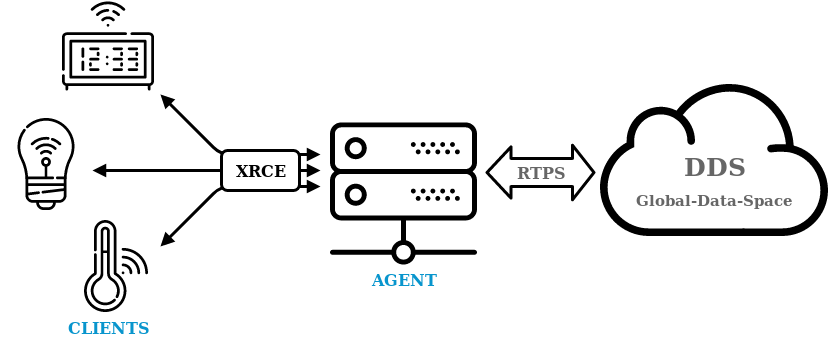
\includegraphics[width=0.95\linewidth]{Img/uxrce_scope.png}
    \caption{structure}\label{f:uxrce}
    \vspace{-0.1in}
\end{figure}

Micro XRCE-DDS is composed by two main elements:
\begin{itemize}
    \item \textbf{Micro XRCE-DDS Agent}: a C++11 out-of-the-box application which implements the XRCE Agent functionality
    \item \textbf{Micro XRCE-DDS Client}: a C99 library which implements the XRCE Client side functionality
\end{itemize}

In addition, Micro XRCE-DDS uses other two components:
\begin{itemize}
    \item \textbf{Micro CDR}: a \underline{de/serialization engine} used in the Client library
    \item \textbf{Micro XRCE-DDS Gen}: a code generator tool used for generating Micro CDR de/serialization functions and Client apps examples from IDL sources.
\end{itemize}

\subsection{Main Features}
\textbf{1. Low Resource Consumption}: As it was mentioned above, Micro XRCE-DDS is focused on microcontroller applications. Therefore, the design and implementation of this middleware have been carried out taking into account the memory constraints of this kind of devices. A proof of this is the fact that the XRCE Client is completely \underline{dynamic memory free}. From the point of view of the memory footprint, the latest version of this library has a memory consumption of less than 75 KB of Flash memory and around 3 KB of RAM for a complete publisher and subscriber application handling messages sizes on the order of 512 B. For more detailed information on the memory consumption as a function of message size, entity number and internal memory management of the middleware library, please refer to the \href{https://micro.ros.org/docs/concepts/middleware/memo_prof/}{Micro XRCE-DDS memory profiling section}. Moreover, this library is highly configurable thanks to a profile concept that enables to choose, add or remove some features in configuration time. That allows customizing the XRCE Client library size, if there are features that are not used. There are several definitions for configuring and building the Client library at compile-time. These definitions allow to create a version of the library according to the application requirements, and can be modified in the client.config file. For incorporating the desired configuration, it is necessary to run the cmake command every time the definitions change.

\textbf{2. Multi-Transport Support}: As part of the profiles discussed in the previous section, the user can choose between several transport layers to communicate the Clients with the Agent. Indeed, in contrast to other IoT middleware such as MQTT and CoaP, which work over only a particular transport layer, XRCE supports multiple transport protocols natively. In particular, the latest version of Micro XRCE-DDS support: UDP, TCP and a custom Serial transport protocol. Apart from this, Micro XRCE-DDS has a transport interface for both Agent and Client which allows to implement custom transports in a straightforward manner. This makes the port of Micro XRCE-DDS to different platforms and the addition of new transports a seamless task that any user can undertake.

\textbf{3. Multi-Platform Support}: The XRCE Client supports FreeRTOS, Zephyr and NuttX as embedded RTOS. Moreover, it also runs on Windows and Linux. On the other hand, the XRCE Agent supports Windows and Linux.

\textbf{4. QoS support}: The XRCE Client library allows the user to use two different approaches for creating DDS entities in the XRCE Agent: By XML (the default option), By reference. When using the default option, users are enabled to create entities either in Reliable or Best-Effort mode, with the XML files written and stored on the Client side. But these QoS configurations may not fit some users’ requirements. For these cases, Micro XRCE-DDS allows to create entities directly on the Agent, where the user can write custom XML QoS as in DDS. Each entity available on the Agent will be associated to a label, so that the Clients can to create the entities they need for the communication by just referring to these labels. Additionally, using references will also reduce the memory consumption of the Client inside the MCU. This is because the reference approach allows avoiding to build the parts of the code where XMLs are stored.

\subsection{Micro XRCE-DDS Client}
The Micro XRCE-DDS Clients\footnote{Github: https://github.com/eProsima/Micro-XRCE-DDS-Client} are lightweight entities meant to be compiled on eXtremely Resource Constrained Environments.
\begin{figure}[htb!]
    \centering
    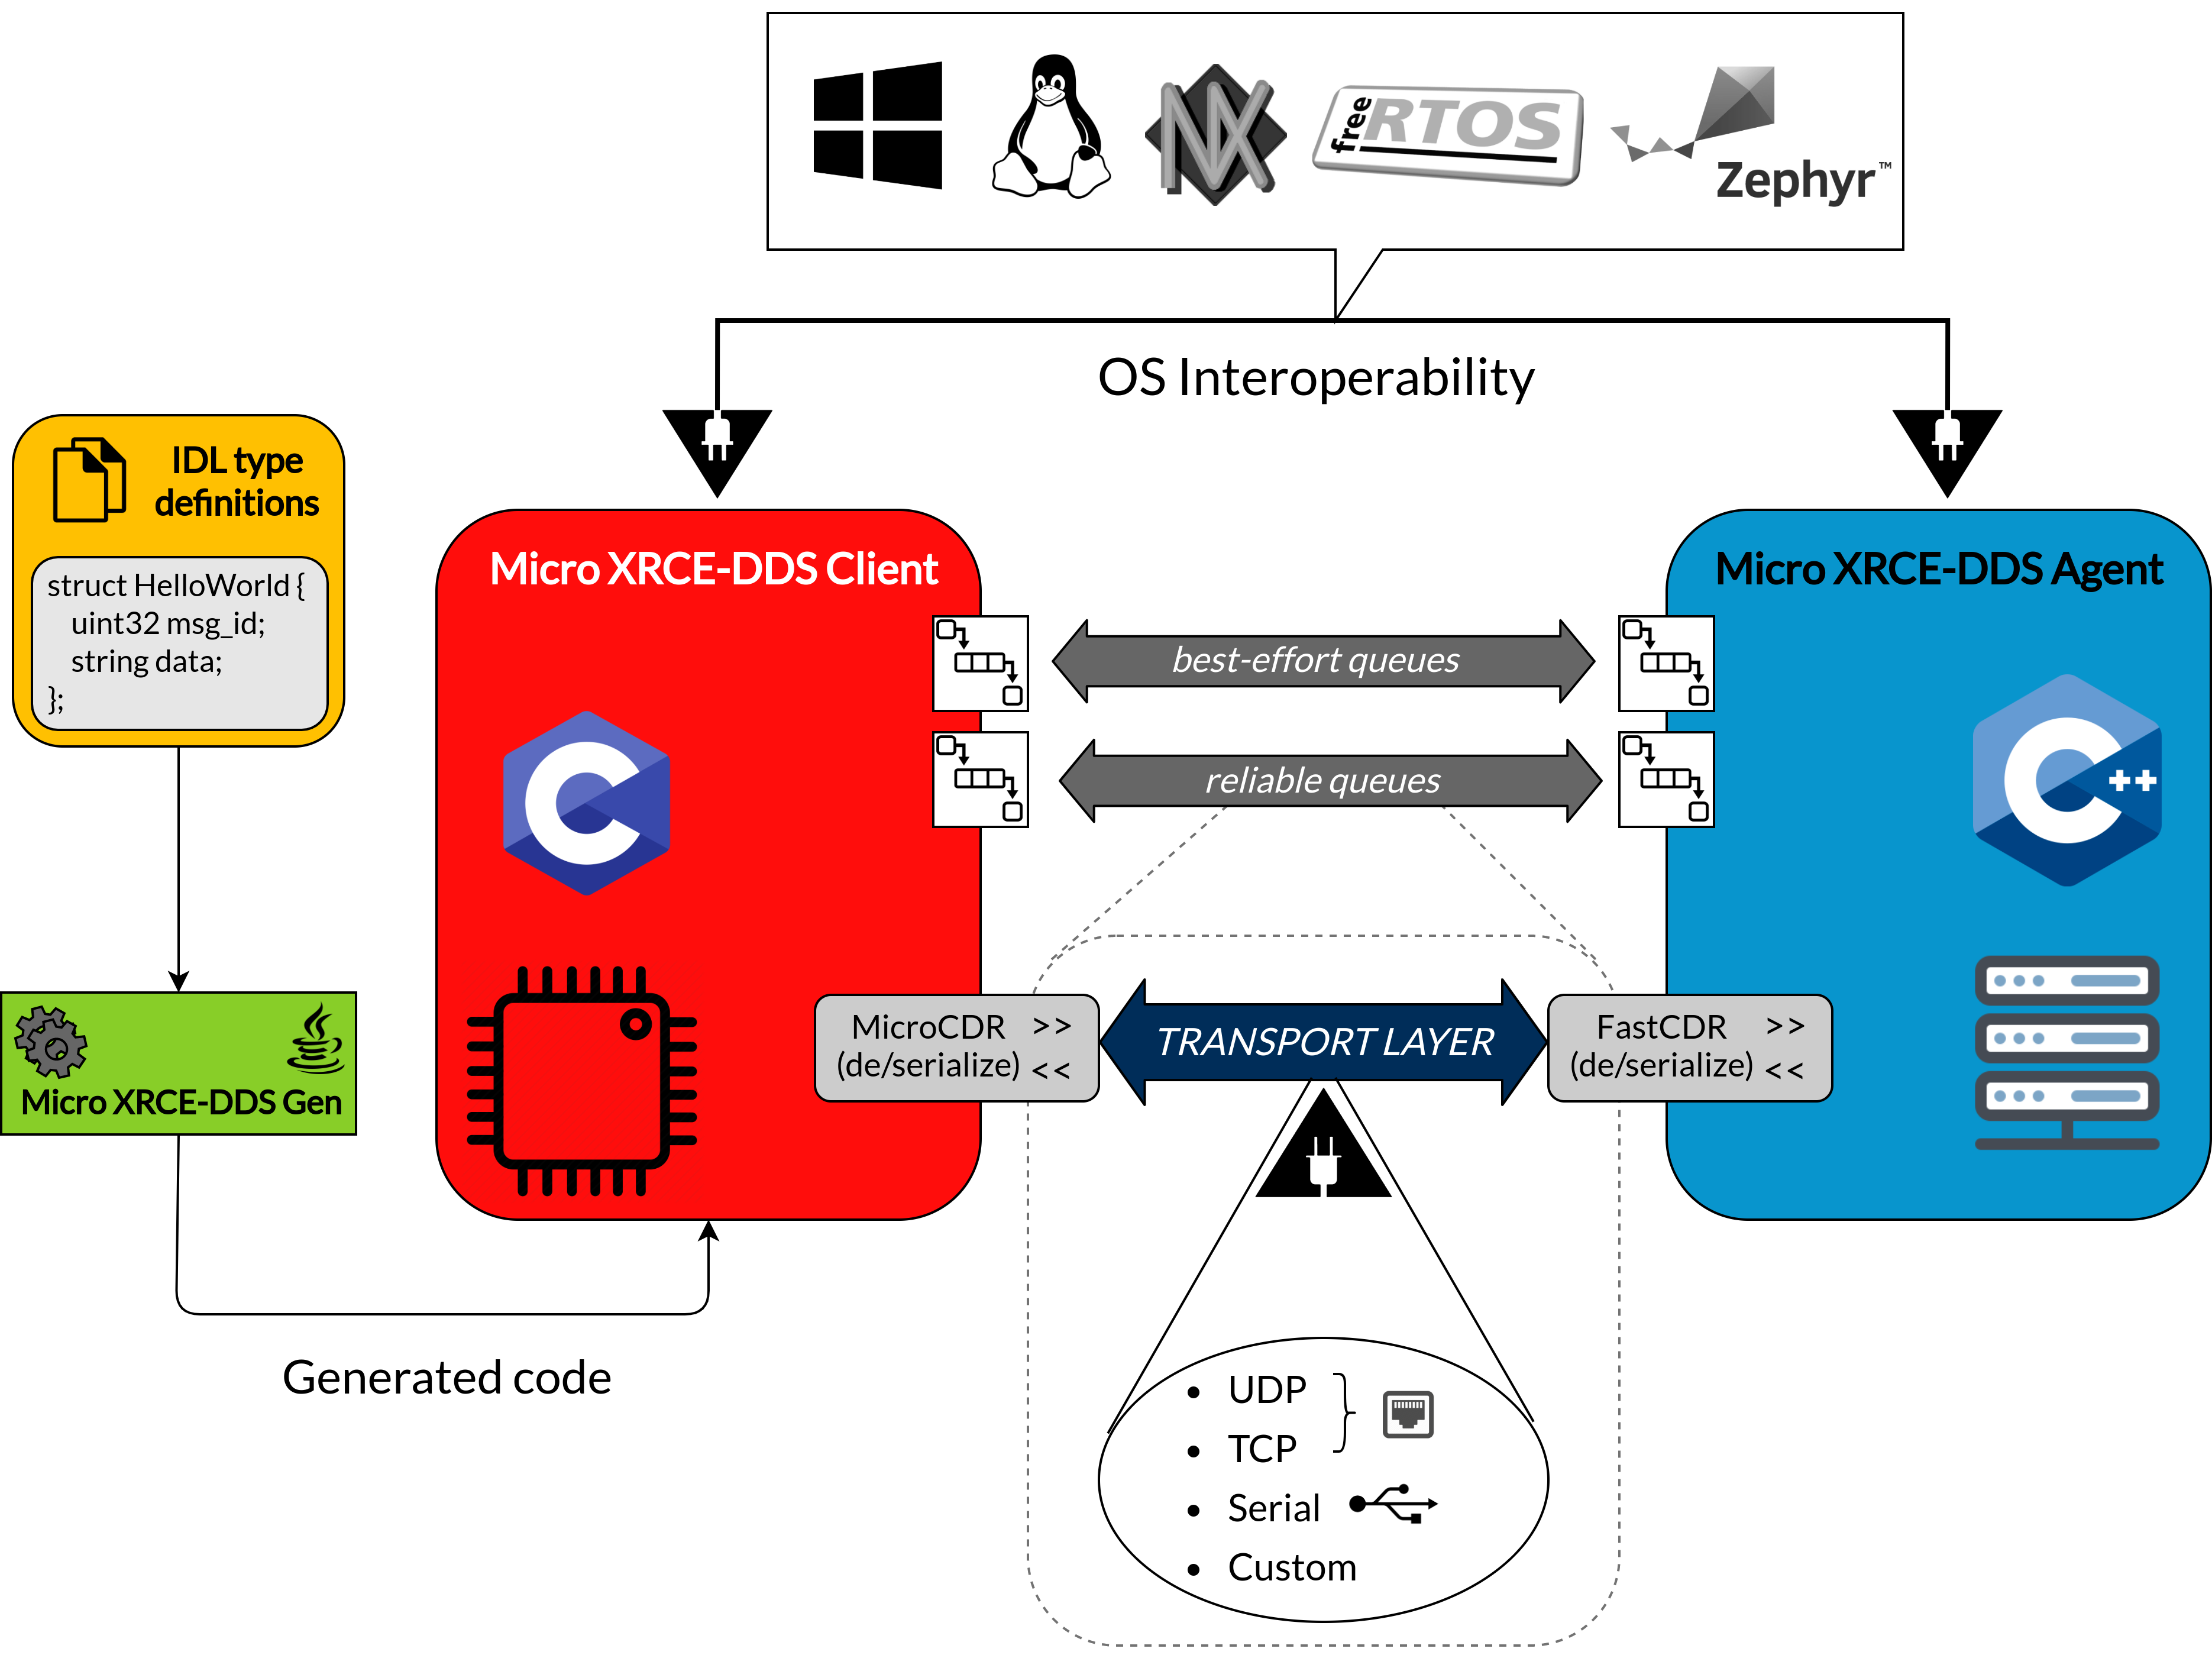
\includegraphics[width=0.95\linewidth]{Img/General.png}
    \caption{structure}\label{f:general}
    \vspace{-0.1in}
\end{figure}

The Micro XRCE-DDS Clients request operations to the Agent to publish and/or subscribe to topics in the DDS global dataspace. Remote procedure calls, as defined by the DDS-RPC standard, are also supported, allowing Clients to communicate in the DDS dataspace according to a request/reply paradigm. The Agents process these requests and send back a response with the operation status result and with the requested data, in the case of subscribe/reply operations. The communication in the DDS world is mediated by a dedicated ProxyClient in charge of creating the DDS Entities requested by the Clients, such as Participants, Topics, Publishers, and Subscribers, which can interact with the DDS Global dataspace.
\begin{figure}[htb!]
    \centering
    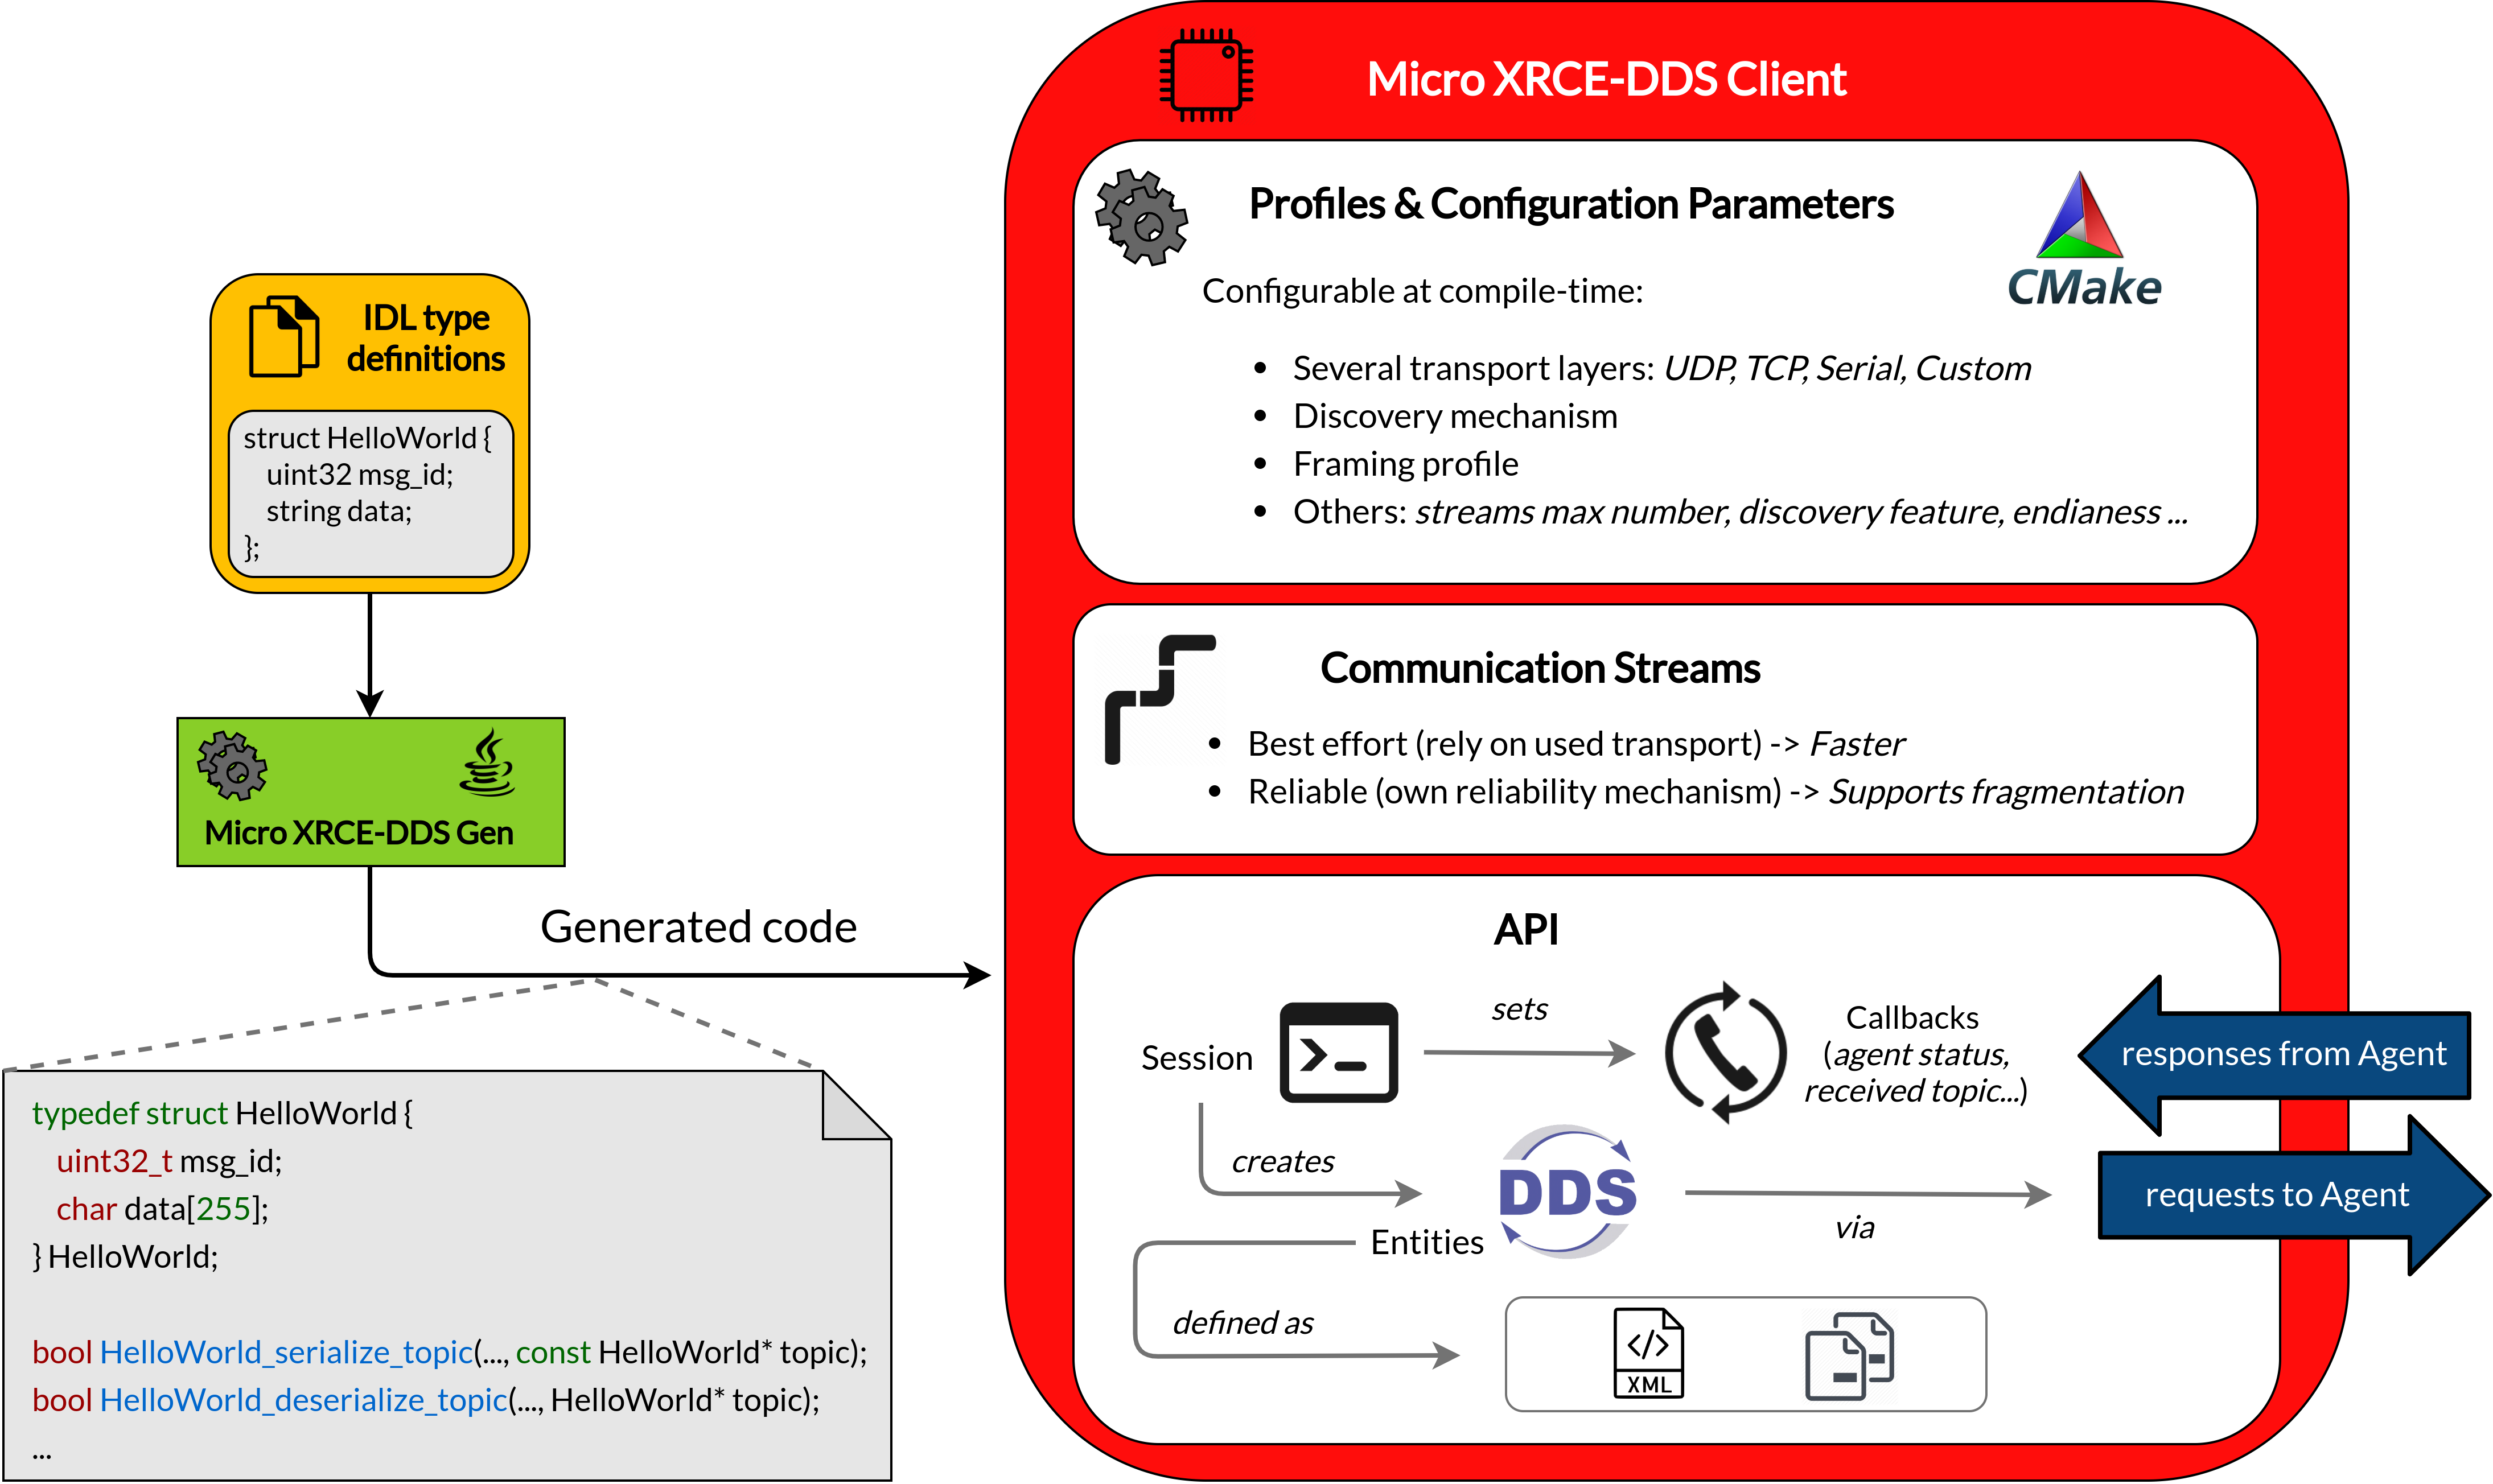
\includegraphics[width=0.95\linewidth]{Img/Client.png}
    \caption{client}\label{f:client}
    \vspace{-0.1in}
\end{figure}
eProsima Micro XRCE-DDS provides the user with a C API to create Micro XRCE-DDS Clients applications. The library can be configured at compile-time via a set of CMake flags allowing to enable or disable some profiles before compilation, and to manipulate several parameters controlling some of the library's functionalities, which in turn allow tuning the library size.

The communication between a Micro XRCE-DDS Client and a Micro XRCE-DDS Agent is achieved by means of several kinds of built-in transports: UDPv4, UDPv6, TCPv4, TCPv6 and Serial communication. In addition, there is the possibility for the user to generate its own Custom transport.

\subsection{Micro XRCE-DDS Agent} 
The Micro XRCE-DDS Agent\footnote{Github: https://github.com/eProsima/Micro-XRCE-DDS-Agent} is a broker which bridges the Clients with the DDS world.
\section{USED POSIX API}
\chapter{Implementation of uROS}
\section{RCLC}
This repository provides the \textit{rclc} package, which complements the ROS Client Support Library (\textit{rcl}) to make up a complete ROS 2 client library for the C programming language. That is, \textit{rclc} does not add a new layer of types on top of \textit{rcl} (like rclcpp and rclpy do) but only provides convenience functions that ease the programming with the \textit{rcl} types. New types are introduced only for concepts that are missing in \textit{rcl}, most important an Executor and a Lifecycle Node.

The API of the RCLC-Executor can be divided in several phases: \textbf{Configuration}, \textbf{Running} and \textbf{Clean-Up}.

\subsection{Configuration Phase}
During the configuration phase, the user shall define: the total number of callbacks, trigger condition (optional, default: ANY), data communication semantics (optional, default RCLCPP) and the processing sequence of the callbacks.
\subsubsection{\api{rclc\_executor\_t * rclc\_get\_zero\_initialized\_executor()}}
Returns a zero initialized executor object.

\subsubsection{\api{rclc\_executor\_init(rclc\_executor\_t * executor, rcl\_context\_t * context, const size\_t number\_of\_handles, const rcl\_allocator\_t * allocator)}}
As the Executor is intended for embedded controllers, dynamic memory management is crucial. Therefore at initialization of the RCLC-Executor, the user defines the total number of handles \textit{number\_of\_handles}. \textbf{A handle is a term for subscriptions, timers, services, clients and guard conditions.} The necessary dynamic memory will be allocated only in this phase and no more memory in the running phase. The corresponding wait-set is allocated in the first execution of the spin-method or in the optional call to \textit{rclc\_executor\_prepare}. This makes this Executor static in the sense, that during runtime no heap allocations occur. You can add, however, at runtime as many handles, e.g. subscriptions, to the executor until the maximum number of handles is reached. The \textit{context} is the RCL context, and \textit{allocator} points to a memory allocator.
\begin{figure}[htb!]
    \centering
    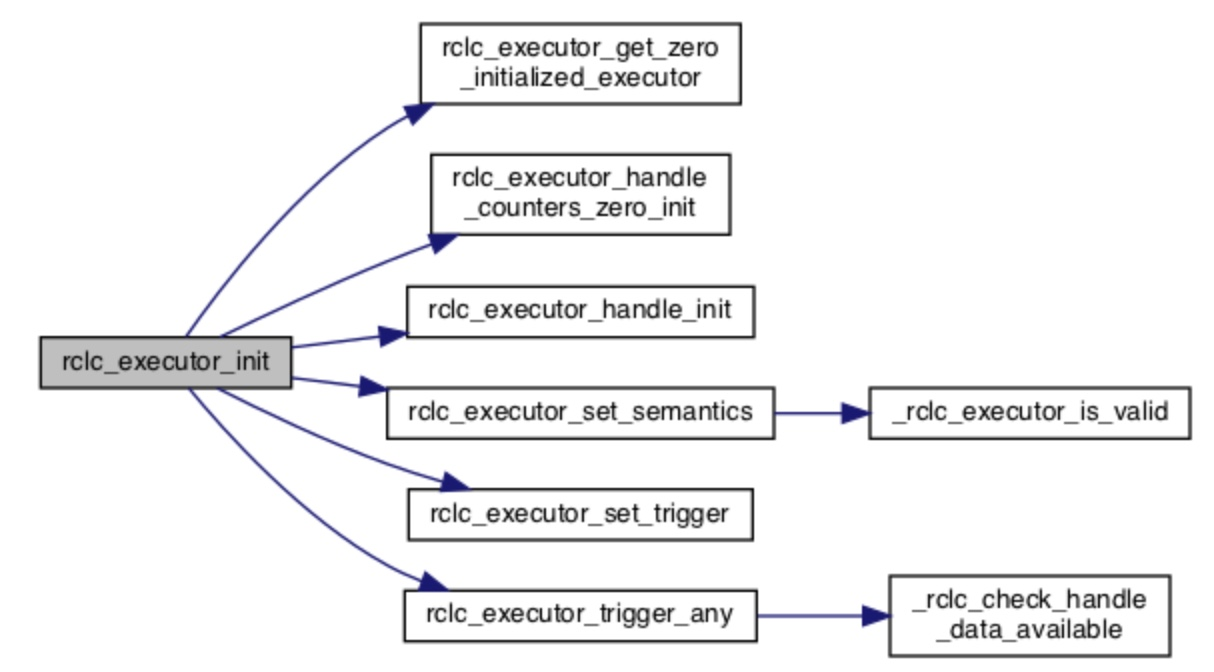
\includegraphics[width=0.95\linewidth]{Img/graph/rclc/executor_init.jpg}
    \caption{executor\_init call}
    \vspace{-0.1in}
\end{figure}

\begin{figure}[htb!]
    \centering
    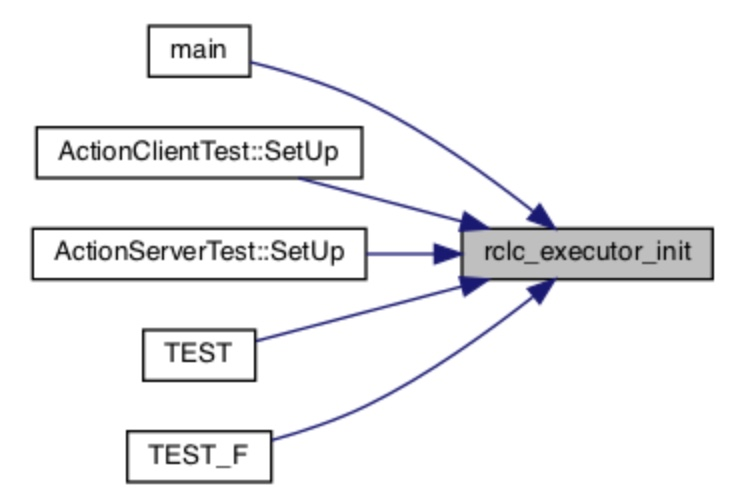
\includegraphics[width=0.75\linewidth]{Img/graph/rclc/executor_init_caller.jpg}
    \caption{executor\_init caller}
    \vspace{-0.1in}
\end{figure}


\subsubsection{\api{rclc\_executor\_set\_timeout(rclc\_executor\_t * executor, const uint64\_t timeout\_ns)}}
The timeout in nano-seconds \textit{timeout\_ns} for waiting for new data from the DDS-queue is specified in \api{rclc\_executor\_set\_timeout()} (this is the timeout parameter for \api{rcl\_wait()}).

\subsubsection{\api{rclc\_executor\_set\_semantics(rclc\_executor\_t * executor, rclc\_executor\_semantics\_t semantics)}}
The \textbf{data communication semantics} can either be \textit{RCLCPP}(default) or \textit{LET}.

To be compatible with ROS 2 rclcpp Executor, the existing rclcpp semantics is implemented with the option \textit{RCLCPP}. That is, with the spin-function the DDS-queue is constantly monitored for new data (\api{rcl\_wait()}). If new data becomes available, then it is fetched from DDS (\api{rcl\_take()}) immediately before the callback is executed. All callbacks are processed in the user-defined order, this is the only difference to the rclcpp Executor, in which the order can not be defined by the user.

The LET semantics is implemented such that at the beginning of processing, all available data is fetched (\api{rcl\_take()}) and buffered and then the callbacks are processed in the pre-defined operating on the buffered copy.

\subsubsection{\api{rclc\_executor\_set\_trigger(rclc\_executor\_t * executor, rclc\_executor\_trigger\_t trigger\_function, void * trigger\_object)}}
The trigger condition \api{rclc\_executor\_set\_trigger} defines when the processing of the callbacks shall start. For convenience some trigger conditions have been defined:
\begin{itemize}
    \item \textit{rclc\_executor\_trigger\_any(default)}: start executing if any callback has new data
    \item \textit{rclc\_executor\_trigger\_all}: start executing if all callbacks have new data
    \item \textit{rclc\_executor\_trigger\_one(\&data)}: start executing if \textit{data} has been received
    \item \textit{rclc\_executor\_trigger\_always}: returns always true, that is every time the Executor spins, the processing of the callbacks is invocated. For example with \textit{spin\_period} and this trigger condition as well as specifying all callbacks of subscriptions being called as \textit{ALWAYS}, a fixed period execution of all callbacks can be implemented, irrespective whether new data is available or not.
    \item \textit{user\_defined\_function}: the user can also define its own function with more complex logic
\end{itemize}

With the \textit{rclc\_executor\_trigger\_one} trigger, the handle to trigger is specified with \textit{trigger\_object}. In the other cases of the trigger conditions this parameter shall be \textit{NULL}.

\subsubsection{\api{rclc\_executor\_add\_subscription(rclc\_executor\_t * executor, rcl\_subscription\_t * subscription, void * msg, rclc\_subscription\_callback\_t callback, rclc\_executor\_handle\_invocation\_t invocation)} AND \api{rclc\_executor\_add\_timer( rclc\_executor\_t * executor, rcl\_timer\_t * timer)}}
To add handles to the Executor, the functions \api{rclc\_executor\_add\_subscription()} for subscriptions and \api{rclc\_executor\_add\_timer()} for timers. The order in which these functions are called, defines later the sequential processing order during runtime.

For adding a subscription, the rcl subscription handle \textit{subscription}, a pointer an allocated message \textit{msg}, the message callback \textit{callback} and an invocation option \textit{invocation} need to be specified. \textbf{The invocation option specifies}, whether the callback shall be executed only if new data is available (\textit{ON\_NEW\_DATA}) or if the callback shall always be executed (\textit{ALWAYS}). The second option is useful for example when the callback is expected to be called at a fixed rate.

For a timer, only the rcl timer object \textit{timer} is needed.

\subsubsection{\api{rclc\_executor\_prepare(rclc\_executor\_t * executor)}}
The function \api{rclc\_executor\_prepare} prepares the internal RCL wait set allocating the required dynamic memory. Its use is optional becouse it also will be checked in the spin functions. If used and no entities are added to the executor during running phase, no dynamic allocations are guaranteed during the running phase.

\subsection{Running Phase}
\subsubsection{\apiarg{rclc\_executor\_spin\_some}{rclc\_executor\_t * executor, const uint64\_t timeout\_ns}}
The function \api{rclc\_executor\_spin\_some} checks for new data from the DDS queue once. \textbf{It first copies all data into local data structures and then executes all handles according the specified order.} This implements the LET semantics. Note that memory is dynamically allocated within rcl-layer, when DDS queue is accessed with \api{rcl\_wait\_set\_init()}.

The static-LET executor performs the following actions:
\begin{itemize}
    \item [(1)] initializes the \texttt{wait\_set} with all handle of the array executor->handles
    \item [(2)] waits for new data from DDS queue with \api{rcl\_wait()} with timeout executor->timeout\_ns
    \item [(3)] takes all ready handles from the \texttt{wait\_set} with \api{rcl\_take()}
    \item [(4)] processes all handles in the order, how they were added to the executor with the respective add-functions by calling respective callback (thus implementing first-read, process, semantic of LET)
\end{itemize}

\begin{figure}[htbp!]
    \vspace{-0.3in}
    \centering
    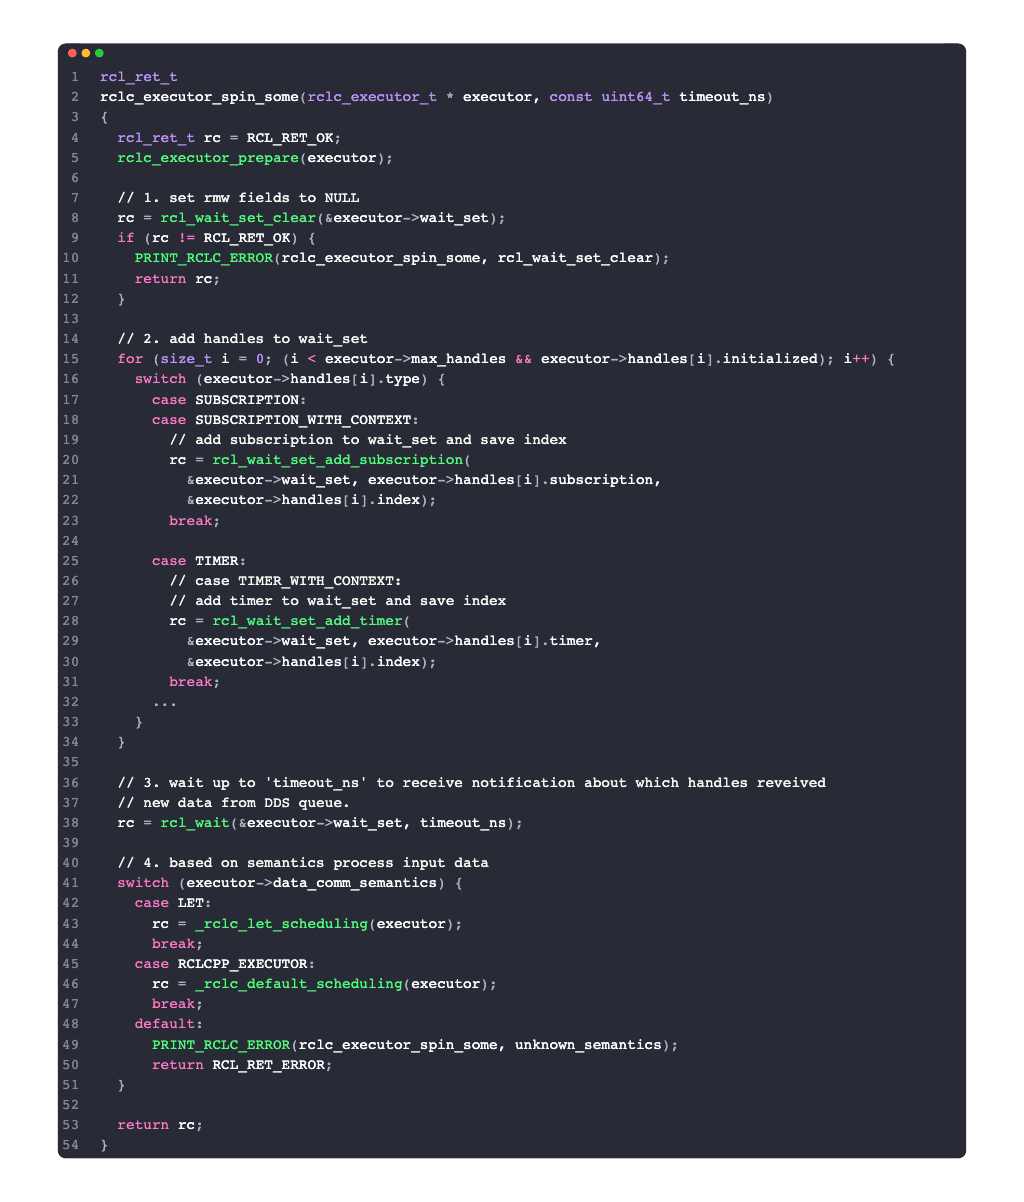
\includegraphics[width=1\linewidth]{Img/code/rclc/rclc_executor_spin_some.png}
    \caption{rclc\_executor\_spin\_some code}
    \vspace{-0.1in}
\end{figure}

\subsubsection{\api{rclc\_executor\_spin(rclc\_executor\_t * executor)}}
The function \api{rclc\_executor\_spin} calls \api{rclc\_executor\_spin\_some} indefinitely as long as the ROS system is alive. This might create a high performance load on your processor.

\subsubsection{\api{rclc\_executor\_spin\_period(rclc\_executor\_t * executor, const uint64\_t period)}}
The function \api{rclc\_executor\_spin\_period} calls \api{rclc\_executor\_spin\_some} periodically (as defined with the argument period) as long as the ROS system is alive.

\subsubsection{\apiarg{rclc\_executor\_spin\_one\_period}{rclc\_executor\_t * executor, const uint64\_t period}}
This is a function used by \api{rclc\_executor\_spin\_period} to spin one time. The purpose is to test the accuracy of the \api{spin\_period} function in the unit tests.

\subsection{Clean-Up Phase}
\subsubsection{\apiarg{rclc\_executor\_fini}{}}
The function \api{rlce\_executor\_fini} frees the dynamically allocated memory of the executor.

\subsection{RCL convenience functions}
The rclc package also provides a number of convenience functions, which make it easier to create the RCL-objects \textit{rcl\_node\_t}, \textit{rcl\_subscription\_t}, \textit{rcl\_timer\_t} and \textit{rcl\_publisher\_t}. Convenience functions:
\begin{itemize}
    \item \api{rclc\_support\_init()}
    \item \api{rclc\_support\_init\_with\_options()}
    \item \api{rclc\_support\_fini()}
    \item \api{rclc\_node\_init\_default()}
    \item \api{rclc\_publisher\_init\_default()}
    \item \api{rclc\_subscription\_init\_default()}
    \item \api{rclc\_timer\_init\_default()}
\end{itemize}

\subsection{Examples}
\subsubsection{Example of real-time embedded application use-case}
In embedded systems, real-time behavior is approached by using the time-triggered paradigm, which means that the processes are periodically activated. Processes can be assigned priorities to allow pre-emptions. Figure~\ref{fig:sch1} shows an example, in which three processes with fixed periods are shown. The middle and lower process are preempted multiple times depicted with empty dashed boxes. To each process one or multiple tasks can be assigned, as shown in Figure~\ref{fig:sch2}. These tasks are executed sequentially, which is often called cooperative scheduling.
\begin{figure*}[t!]
    \begin{minipage}[t]{0.5\textwidth}
        \setcaptionwidth{2in}
        %\hspace{0pt}
        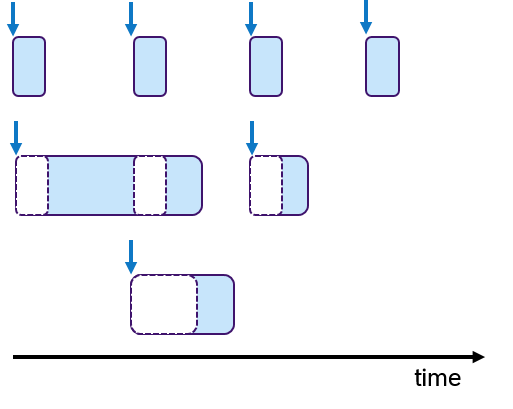
\includegraphics[scale = 0.8]{Img/scheduling_01.png}
        \caption{Fixed periodic preemptive scheduling}
        \label{fig:sch1} %\vspace{-10pt}
    \end{minipage}
    \begin{minipage}[t]{0.5\textwidth}
        \setcaptionwidth{2in}
        %\hspace{0pt}
        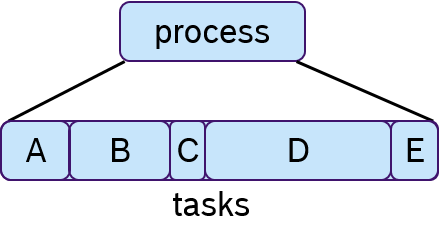
\includegraphics[scale = 0.8]{Img/scheduling_02.png}
        \caption{Processes with sequentially executed tasks}
        \label{fig:sch2} %\vspace{-10pt}
    \end{minipage}
\end{figure*}

With sequential execution the co-operative scheduling of tasks within a process can be modeled. The trigger condition is used to periodically activate the process which will then execute all callbacks in a pre-defined order. Data will be communicated using the LET-semantics. Every Executor is executed in its own tread, to which an appropriate priority can be assigned.

In the following example, the Executor is setup with 4 handles. We assume a process has three subscriptions \textit{sub1}, \textit{sub2}, \textit{sub3}. The sequential processing order is given by the order as they are added to the Executor. A timer \textit{timer} defines the period. The \textit{trigger\_one} with the parameter timer is used, so that whenever the timer is ready, all callbacks are processed. Finally the data communication semantics LET is defined.

\forget{
\begin{lstlisting}[language=python, caption=real-time embedded application use-case]
#include "rcl_executor/let_executor.h"

// define subscription callback
void my_sub_cb1(const void * msgin)
{
    // ...
}
// define subscription callback
void my_sub_cb2(const void * msgin)
{
    // ...
}
// define subscription callback
void my_sub_cb3(const void * msgin)
{
    // ...
}

// define timer callback
void my_timer_cb(rcl_timer_t * timer, int64_t last_call_time)
{
    // ...
}

// necessary ROS 2 objects
rcl_context_t context;
rcl_node_t node;
rcl_subscription_t sub1, sub2, sub3;
rcl_timer_t timer;
rcle_let_executor_t exe;

// define ROS context
context = rcl_get_zero_initialized_context();
// initialize ROS node
rcl_node_init(&node, &context,...);
// create subscriptions
rcl_subscription_init(&sub1, &node, ...);
rcl_subscription_init(&sub2, &node, ...);
rcl_subscription_init(&sub3, &node, ...);
// create a timer
rcl_timer_init(&timer, &my_timer_cb, ... );
// initialize executor with four handles
rclc_executor_init(&exe, &context, 4, ...);
// define static execution order of handles
rclc_executor_add_subscription(&exe, &sub1, &my_sub_cb1, ALWAYS);
rclc_executor_add_subscription(&exe, &sub2, &my_sub_cb2, ALWAYS);
rclc_executor_add_subscription(&exe, &sub3, &my_sub_cb3, ALWAYS);
rclc_executor_add_timer(&exe, &timer);
// trigger when handle 'timer' is ready
rclc_executor_set_trigger(&exe, rclc_executor_trigger_one, &timer);
// select LET-semantics
rclc_executor_data_comm_semantics(&exe, LET);
// spin forever
rclc_executor_spin(&exe);  
\end{lstlisting}}
\begin{figure}[htbp!]
    \centering
    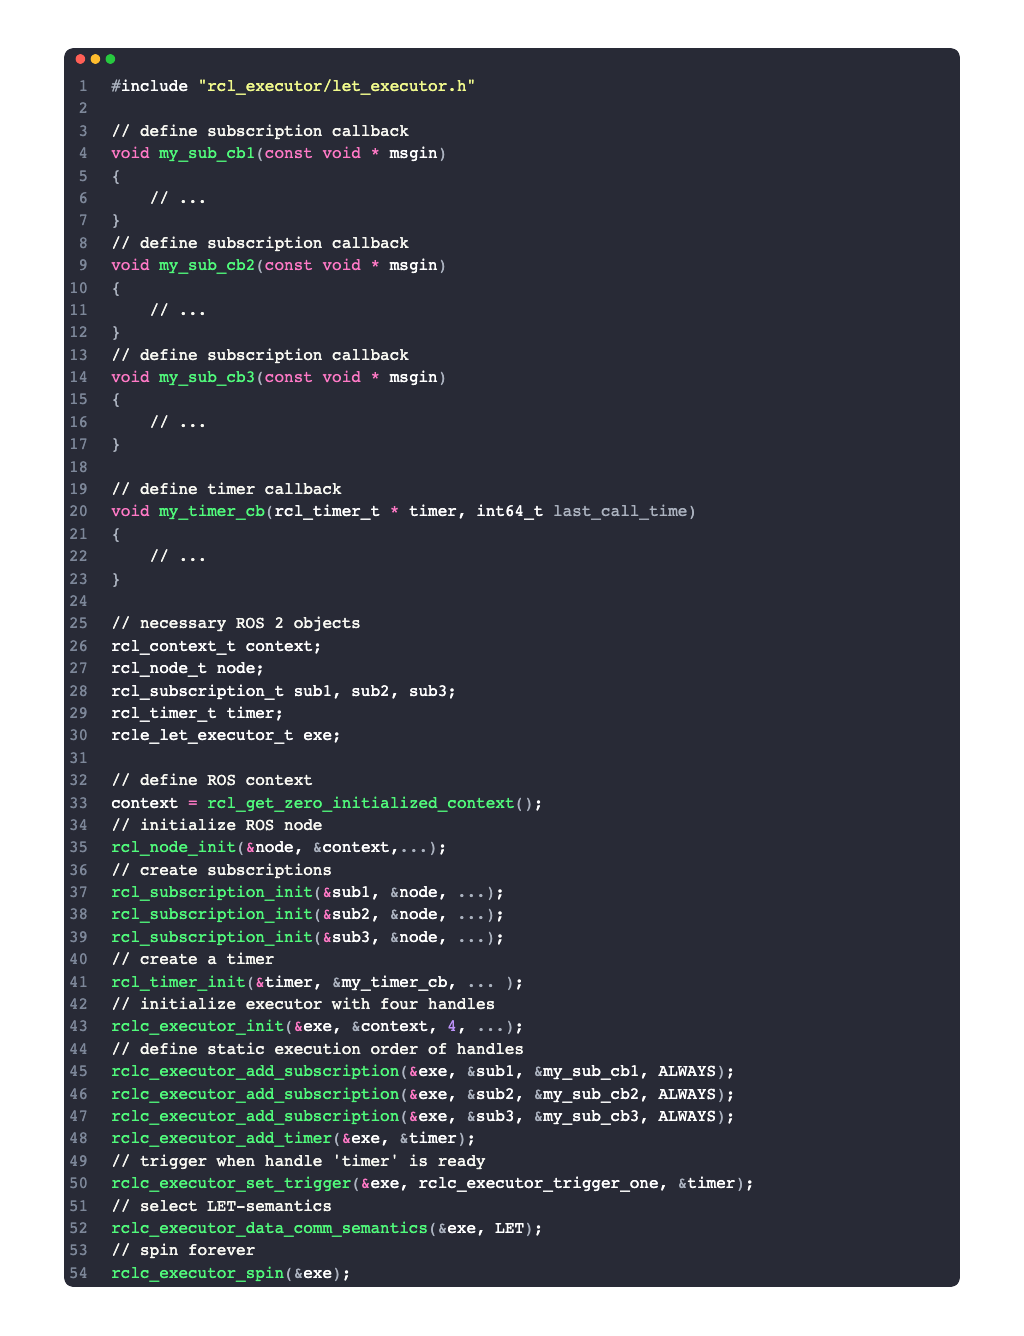
\includegraphics[width=1\linewidth]{Img/code/example1.png}
    \caption{real-time embedded application use-case}\label{f:example1}
    \vspace{-0.1in}
\end{figure}


\subsubsection{Example of sense-plan-act pipeline in mobile robotics}
A common design paradigm in mobile robotics is a control loop, consisting of several phases: A sensing phase to acquire sensor data, a plan phase for localization and path planning and an actuation-phase to steer the mobile robot. Of course, more phases are possible, here these three phases shall serve as an example. Such a processing pipeline is shown in Figure~\ref{f:sensePlanActScheme}. Typically multiple sensors are used to perceive the environment. For example an IMU and a laser scanner. The quality of localization algorithms highly depend on how old such sensor data is when it is processed. Ideally the latest data of all sensors should be processed. One way to achieve this is to execute first all sensor drivers in the sense-phase and then process all algorithms in the plan-phase.
\begin{figure}[htbp!]
    \centering
    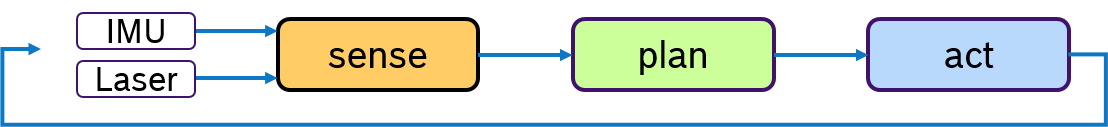
\includegraphics[width=0.75\linewidth]{Img/sensePlanActScheme.png}
    \caption{Multiple sensors driving a Sense-Plan-Act pipeline}\label{f:sensePlanActScheme}
    \vspace{-0.1in}
\end{figure}

In this example we want to realise a sense-plan-act pipeline in a single thread. The trigger condition is demonstrated by activating the sense-phase when both data for the Laser and IMU are available. Three executors are necessary \textit{exe\_sense}, \textit{exe\_plan} and \textit{exe\_act}. The two sensor acquisition callbacks \textit{sense\_Laser} and \textit{sense\_IMU} are registered in the Executor exe\_sense. The trigger condition \textit{ALL} is responsible to activate the sense-phase only when all data for these two callbacks are available. Finally all three Executors are spinning using a while-loop and the \api{spin\_some} function.
\forget{
\begin{lstlisting}[language=python, caption=real-time embedded application use-case]
...
rcl_subscription_t sense_Laser, sense_IMU, plan, act;
rcle_let_executor_t exe_sense, exe_plan, exe_act;
// initialize executors
rclc_executor_init(&exe_sense, &context, 2, ...);
rclc_executor_init(&exe_plan, &context, 1, ...);
rclc_executor_init(&exe_act, &context, 1, ...);
// executor for sense-phase
rclc_executor_add_subscription(&exe_sense, &sense_Laser, &my_sub_cb1, ON_NEW_DATA);
rclc_executor_add_subscription(&exe_sense, &sense_IMU, &my_sub_cb2, ON_NEW_DATA);
rclc_let_executor_set_trigger(&exe_sense, rclc_executor_trigger_all, NULL);
// executor for plan-phase
rclc_executor_add_subscription(&exe_plan, &plan, &my_sub_cb3, ON_NEW_DATA);
// executor for act-phase
rclc_executor_add_subscription(&exe_act, &act, &my_sub_cb4, ON_NEW_DATA);

// spin all executors
while (true) {
    rclc_executor_spin_some(&exe_sense);
    rclc_executor_spin_some(&exe_plan);
    rclc_executor_spin_some(&exe_act);
}
\end{lstlisting}}
\begin{figure}[htbp!]
    \centering
    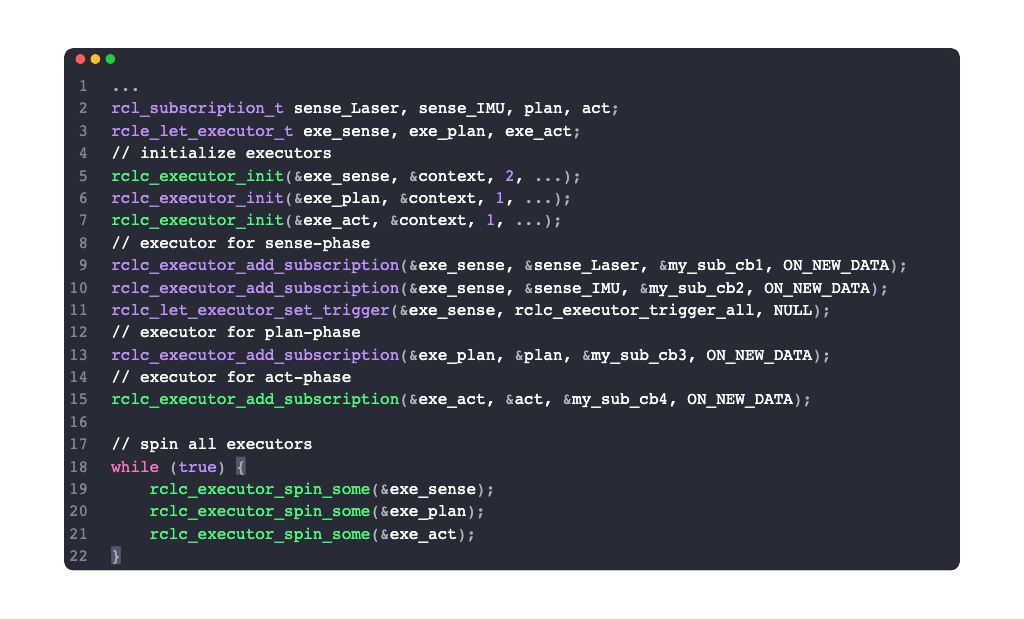
\includegraphics[width=1\linewidth]{Img/code/example2.png}
    \caption{sense-plan-act pipeline in mobile robotics}\label{f:example2}
    \vspace{-0.1in}
\end{figure}


\subsubsection{Example of synchronization of multiple rates}
Often multiple sensors are being used to sense the environment for mobile robotics. While an IMU sensor provides data samples at a very high rate (e.g. 500 Hz), laser scans are available at a much slower frequency (e.g. 10Hz) determined by the revolution time. Then the challenge is, how to deterministically fuse sensor data with different frequencies. This problem is depicted in Figure~\ref{f:sensorFusion_01}.
\begin{figure}[htb!]
    \centering
    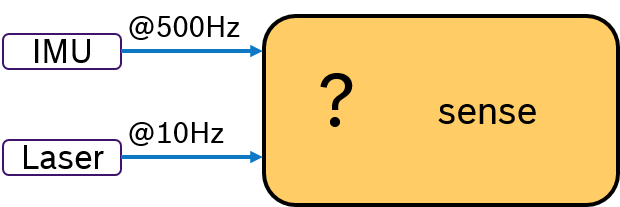
\includegraphics[width=0.75\linewidth]{Img/sensorFusion_01.png}
    \caption{How to deterministically process multi-frequent sensor data}\label{f:sensorFusion_01}
    \vspace{-0.1in}
\end{figure}

An Alternative would be to evaluate the IMU sample and the laser scan by synchronizing their frequency. For example by processing always 50 IMU samples with one laser scan. This approach is shown in Figure \ref{f:sensorFusion_02}. A pre-processing callback aggregates the IMU samples and sends an aggregated message with 50 samples at 10Hz rate. Now both messages have the same frequency. With a trigger condition, which fires when both messages are available, the sensor fusion algorithm can expect always synchronized input data.
\begin{figure}[htb!]
    \centering
    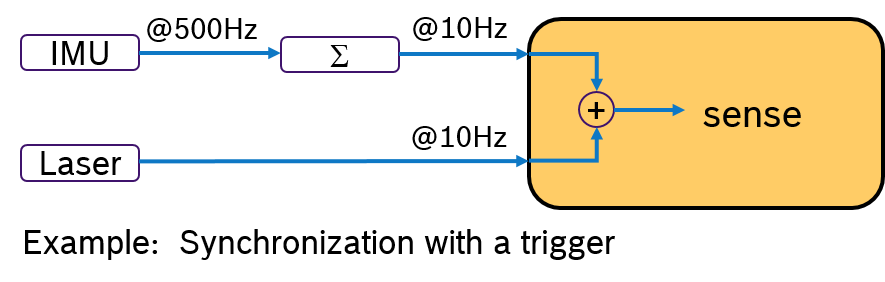
\includegraphics[width=0.75\linewidth]{Img/sensorFusion_02.png}
    \caption{How to deterministically process multi-frequent sensor data}\label{f:sensorFusion_02}
    \vspace{-0.1in}
\end{figure}

The sensor fusion synchronizing the multiple rates with a trigger is shown below.
\forget{
\begin{lstlisting}[language=python, caption=real-time embedded application use-case]
...
rcl_subscription_t aggr_IMU, sense_Laser, sense_IMU;
rcle_let_executor_t exe_aggr, exe_sense;
// initialize executors
rclc_executor_init(&exe_aggr, &context, 1, ...);
rclc_executor_init(&exe_sense, &context, 2, ...);
// executor for aggregate IMU data
rclc_executor_add_subscription(&exe_aggr, &aggr_IMU, &my_sub_cb1, ON_NEW_DATA);
// executor for sense-phase
rclc_executor_add_subscription(&exe_sense, &sense_Laser, &my_sub_cb2, ON_NEW_DATA);
rclc_executor_add_subscription(&exe_sense, &sense_IMU, &my_sub_cb3, ON_NEW_DATA);
rclc_executor_set_trigger(&exe_sense, rclc_executor_trigger_all, NULL);

// spin all executors
while (true) {
    rclc_executor_spin_some(&exe_aggr);
    rclc_executor_spin_some(&exe_sense);
}
\end{lstlisting}}
\begin{figure}[htbp!]
    \centering
    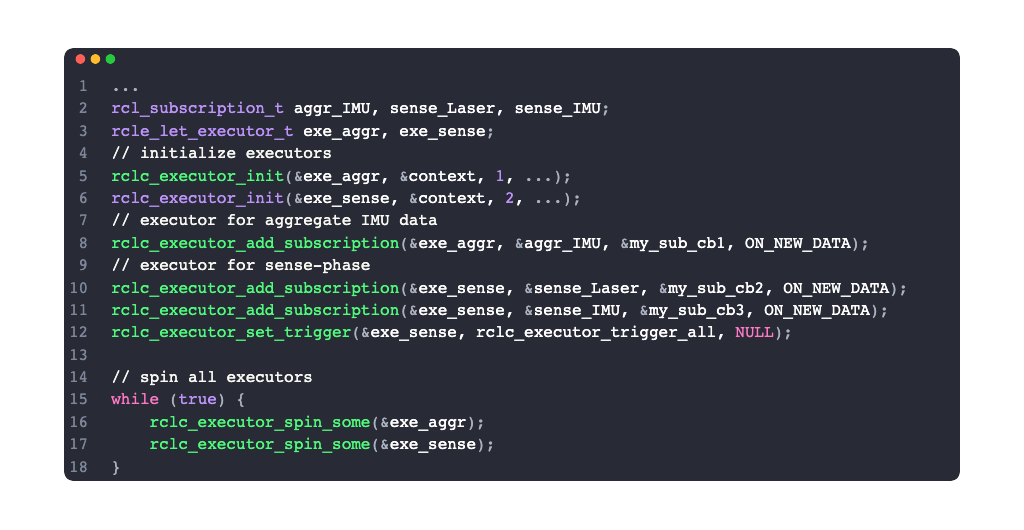
\includegraphics[width=1\linewidth]{Img/code/example3.png}
    \caption{synchronization of multiple rates}\label{f:example3}
    \vspace{-0.1in}
\end{figure}


Another idea would be to actively request for IMU data only when a laser scan is received. This concept is shown in Figure \ref{f:sensorFusion_03}. Upon arrival of a laser scan message, first, a message with aggregated IMU samples is requested. Then, the laser scan is processed and later the sensor fusion algorithm. An Executor, which would support sequential execution of callbacks, could realize this idea.
\begin{figure}[htb!]
    \centering
    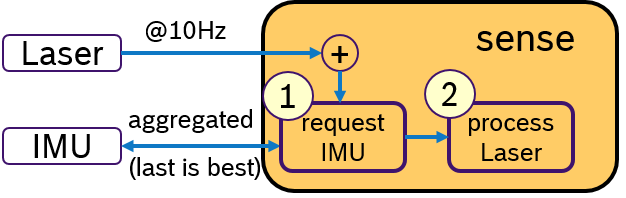
\includegraphics[width=0.75\linewidth]{Img/sensorFusion_03.png}
    \caption{Synchronization of multiple input data with a trigger}\label{f:sensorFusion_03}
    \vspace{-0.1in}
\end{figure}

The setup for the sensor fusion using sequential execution is shown below. Note, that the sequential order is sense\_IMU, which will request the aggregated IMU message, and then sense\_Laser while the trigger will fire, when a laser message is received.
\forget{
\begin{lstlisting}[language=python, caption=real-time embedded application use-case]
...
rcl_subscription_t sense_Laser, sense_IMU;
rcle_let_executor_t exe_sense;
// initialize executor
rclc_executor_init(&exe_sense, &context, 2, ...);
// executor for sense-phase
rclc_executor_add_subscription(&exe_sense, &sense_IMU, &my_sub_cb1, ALWAYS);
rclc_executor_add_subscription(&exe_sense, &sense_Laser, &my_sub_cb2, ON_NEW_DATA);
rclc_executor_set_trigger(&exe_sense, rclc_executor_trigger_one, &sense_Laser);
// spin
rclc_executor_spin(&exe_sense);
\end{lstlisting}}
\begin{figure}[htbp!]
    \centering
    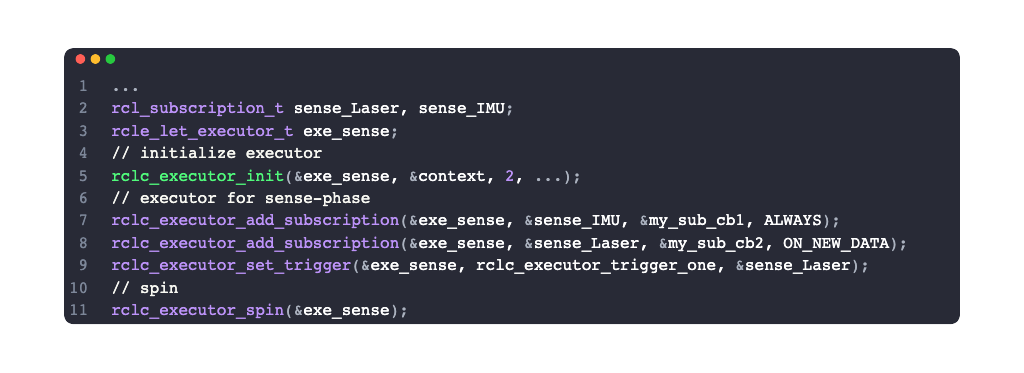
\includegraphics[width=1\linewidth]{Img/code/example32.png}
    \caption{synchronization of multiple rates}\label{f:example32}
    \vspace{-0.1in}
\end{figure}

\subsubsection{Example of high-priority processing path}
Often a robot has to fulfill several activities at the same time. For example following a path and avoiding obstacles. While path following is a permanent activity, obstacle avoidance is triggered by the environment and should be immediately reacted upon. Therefore one would like to specify priorities to activities. This is depicted in Figure \ref{f:highPriorityPath}. Assuming a simplified control loop with the activities sense-plan-act, the obstacle avoidance, which might temporarily stop the robot, should be processed before the planning phase. In this example we assume that these activities are processed in one thread.
\begin{figure}[htb!]
    \centering
    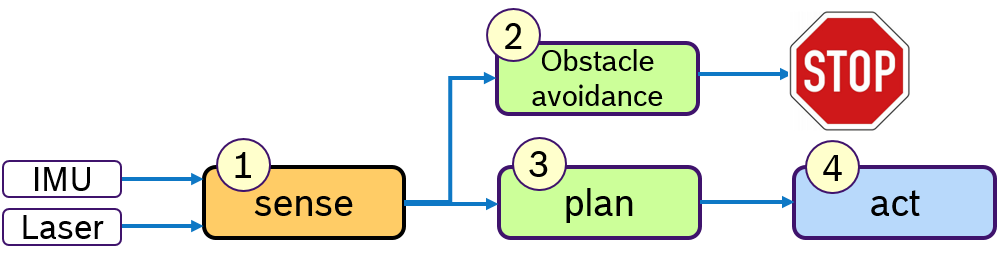
\includegraphics[width=0.75\linewidth]{Img/highPriorityPath.png}
    \caption{Managing high priority path with sequential order}\label{f:highPriorityPath}
    \vspace{-0.1in}
\end{figure}

This example shows the sequential processing order to execute the obstacle avoidance obst\_avoid after the callbacks of the sense-phase and before the callback of the planning phase plan. The control loop is started when a laser message is received. Then an aggregated IMU message is requested, like in the example above. Then all the other callbacks are always executed. This assumes that these callbacks communicate via a global data structure. Race conditions cannot occur, because the callbacks run all in one thread.
\forget{
\begin{lstlisting}[language=python, caption=real-time embedded application use-case]
...
rcl_subscription_t sense_Laser, sense_IMU, plan, act, obst_avoid;
rcle_let_executor_t exe;
// initialize executors
rclc_executor_init(&exe, &context, 5, ...);
// define processing order
rclc_executor_add_subscription(&exe, &sense_IMU, &my_sub_cb1, ALWAYS);
rclc_executor_add_subscription(&exe, &sense_Laser, &my_sub_cb2, ON_NEW_DATA);
rclc_executor_add_subscription(&exe, &obst_avoid, &my_sub_cb3, ALWAYS);
rclc_executor_add_subscription(&exe, &plan, &my_sub_cb4, ALWAYS);
rclc_executor_add_subscription(&exe, &act, &my_sub_cb5, ALWAYS);
rclc_executor_set_trigger(&exe, rclc_executor_trigger_one, &sense_Laser);
// spin
rclc_executor_spin(&exe);
\end{lstlisting}}
\begin{figure}[htbp!]
    \centering
    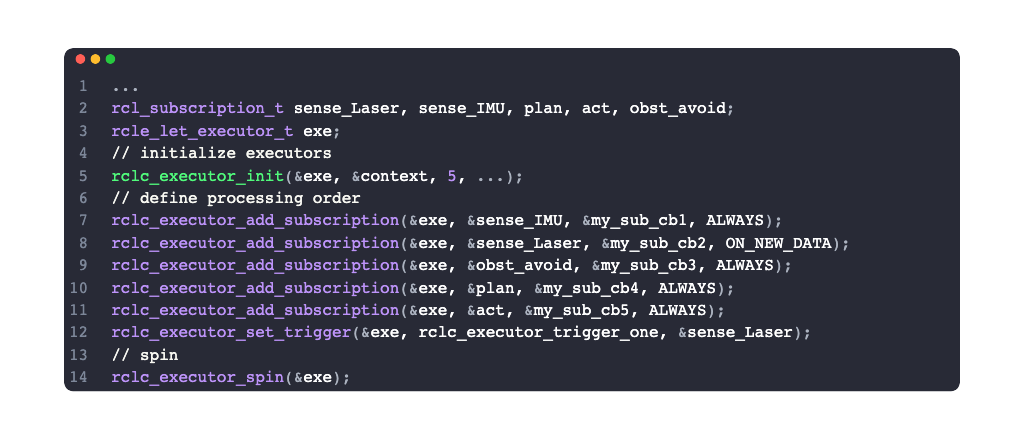
\includegraphics[width=1\linewidth]{Img/code/example4.png}
    \caption{high-priority processing path}\label{f:example4}
    \vspace{-0.1in}
\end{figure}

\subsection{Kernel Functions}
% - NOTE:===========================================================================
\subsubsection{\apiarg{\_rclc\_let\_scheduling}{rclc\_executor\_t * executor}}
\forget{
\begin{figure}[htbp!]
    \centering
    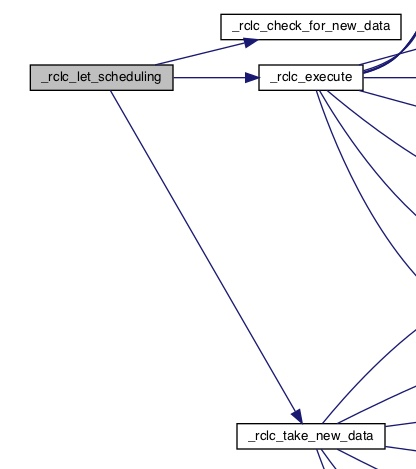
\includegraphics[width=0.3\linewidth]{Img/graph/rclc/let_scheduling_call.jpg}
    \caption{\_rclc\_let\_scheduling call}
    \vspace{-0.1in}
\end{figure}

\begin{figure}[htbp!]
    \centering
    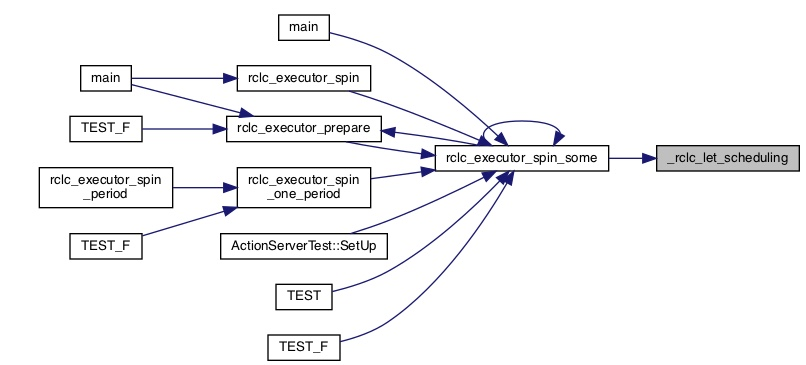
\includegraphics[width=1\linewidth]{Img/graph/rclc/let_scheduling_caller.jpg}
    \caption{\_rclc\_let\_scheduling caller}
    \vspace{-0.1in}
\end{figure}}

\begin{figure}[htbp!]
    \centering
    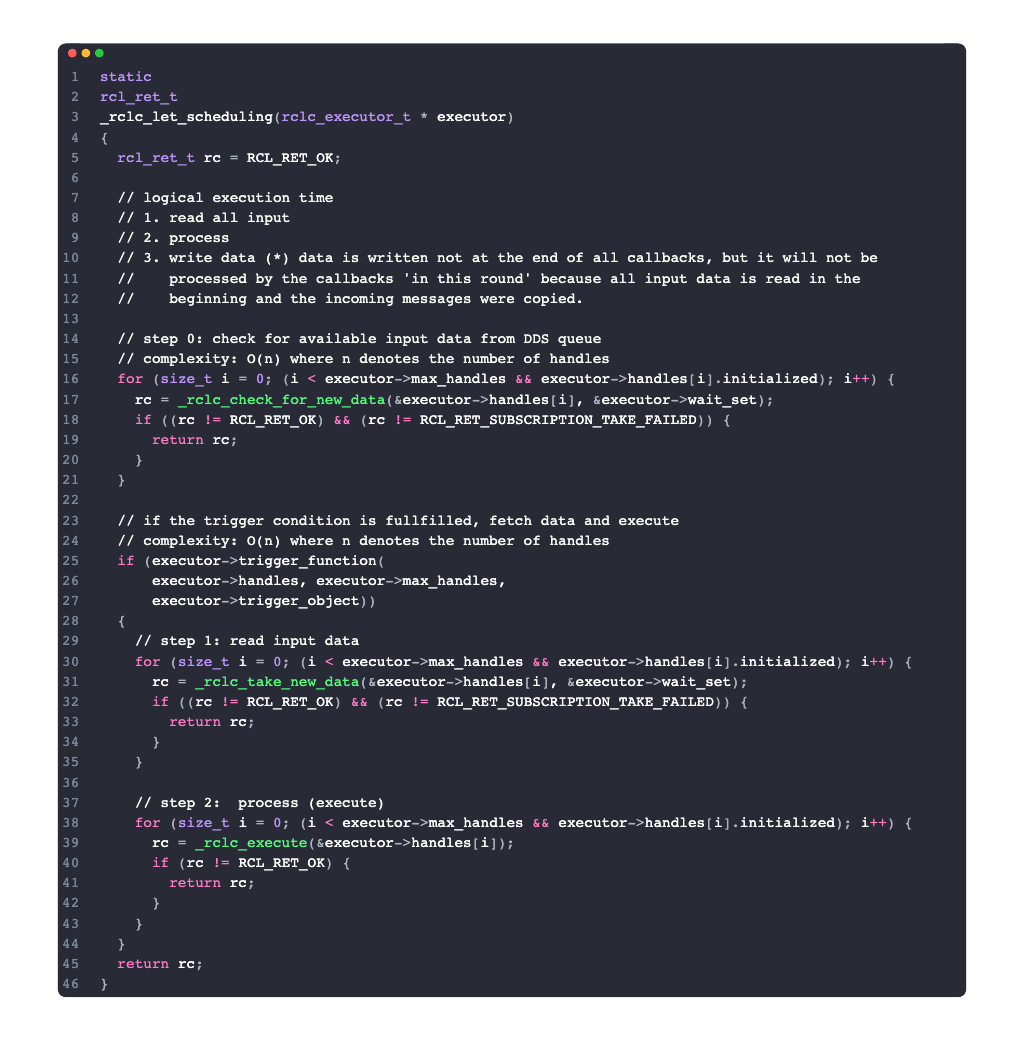
\includegraphics[width=1\linewidth]{Img/code/rclc/_rclc_let_scheduling.png}
    \caption{\_rclc\_let\_scheduling code}
    \vspace{-0.1in}
\end{figure}

% - NOTE:===========================================================================
\subsubsection{\apiarg{\_rclc\_default\_scheduling}{rclc\_executor\_t * executor}}
\begin{figure}[htbp!]
    \centering
    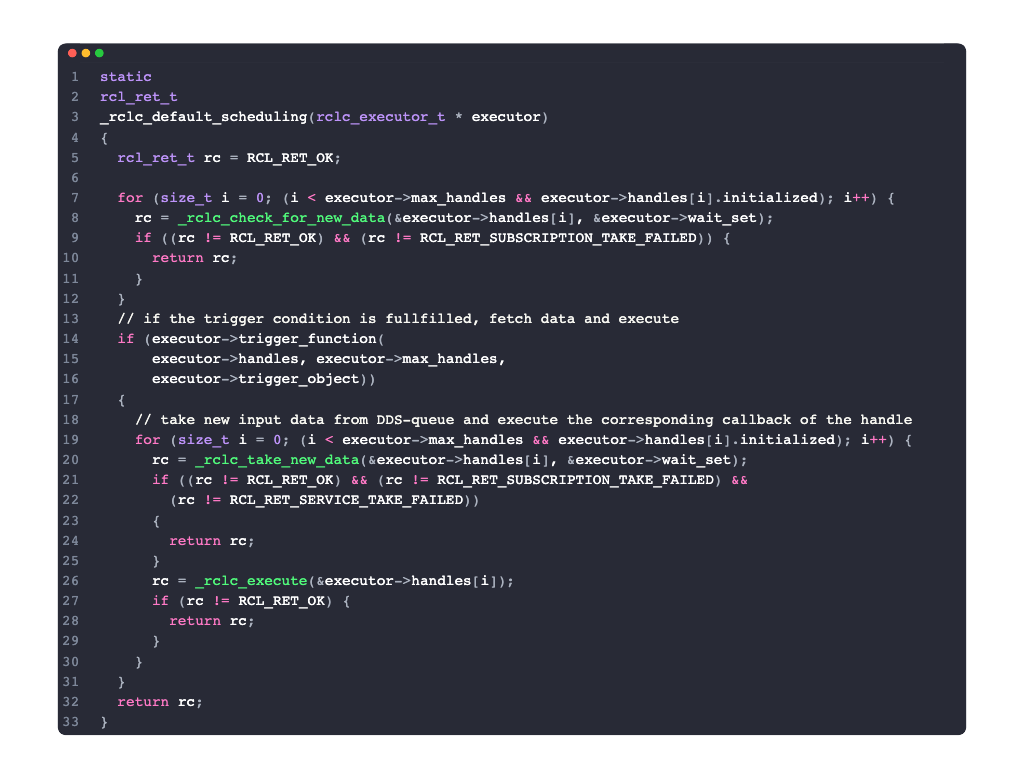
\includegraphics[width=1\linewidth]{Img/code/rclc/_rclc_default_scheduling.png}
    \caption{\_rclc\_let\_scheduling code}
    \vspace{-0.1in}
\end{figure}

% - NOTE:===========================================================================
\subsubsection{\apiarg{\_rclc\_check\_for\_new\_data}{rclc\_executor\_handle\_t * handle, rcl\_wait\_set\_t * wait\_set}}
\begin{figure}[htbp!]
    \centering
    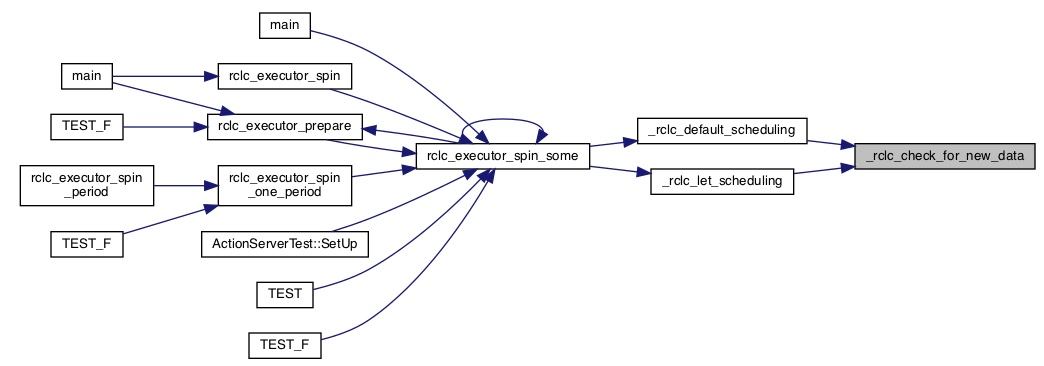
\includegraphics[width=1\linewidth]{Img/graph/rclc/check_for_new_data_caller.jpg}
    \caption{\_rclc\_let\_scheduling caller}
    \vspace{-0.1in}
\end{figure}

\begin{figure}[htbp!]
    \centering
    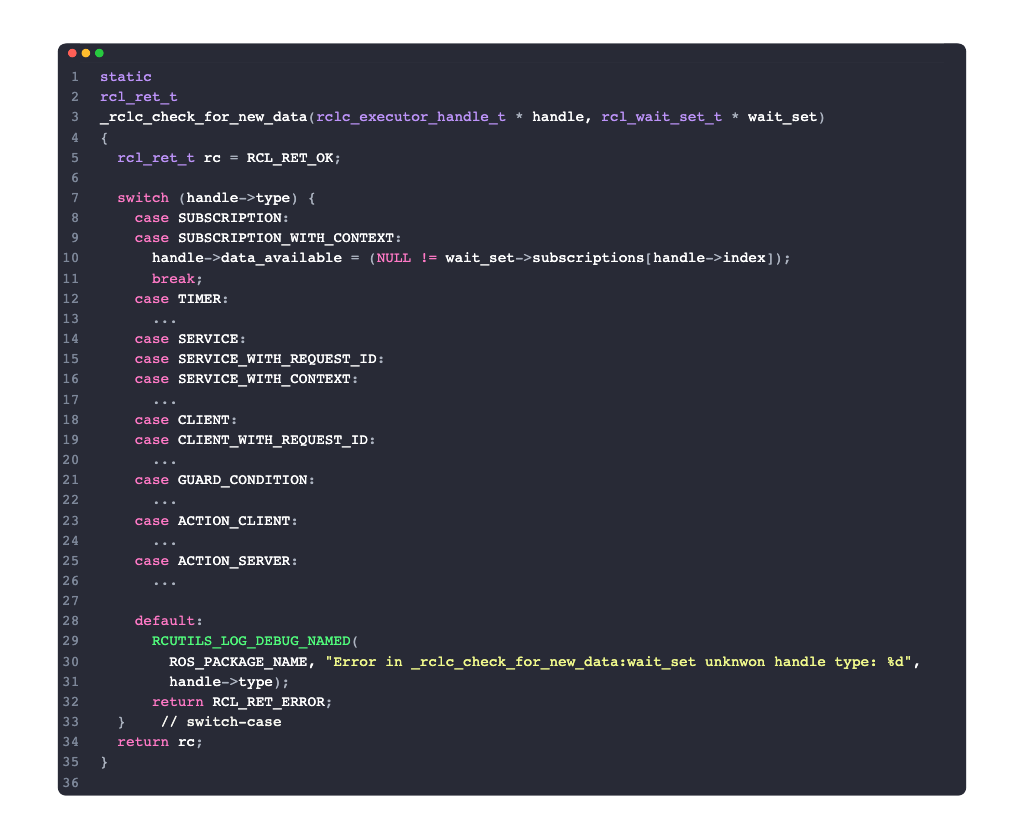
\includegraphics[width=1\linewidth]{Img/code/rclc/_rclc_check_for_new_data.png}
    \caption{\_rclc\_let\_scheduling code}
    \vspace{-0.1in}
\end{figure}

% - NOTE:===========================================================================
\subsubsection{\apiarg{\_rclc\_take\_new\_data}{rclc\_executor\_handle\_t * handle, rcl\_wait\_set\_t * wait\_set}}
\begin{figure}[htbp!]
    \centering
    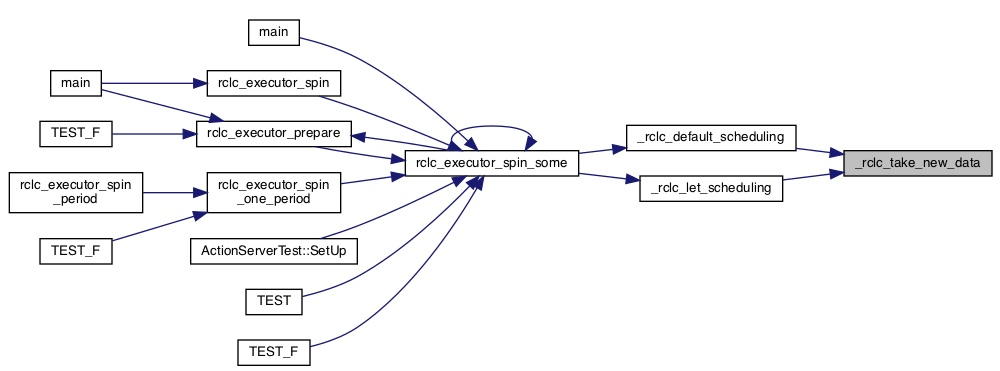
\includegraphics[width=1\linewidth]{Img/graph/rclc/take_new_data_caller.jpg}
    \caption{\_rclc\_let\_scheduling caller}
    \vspace{-0.1in}
\end{figure}

\begin{figure}[htbp!]
    \centering
    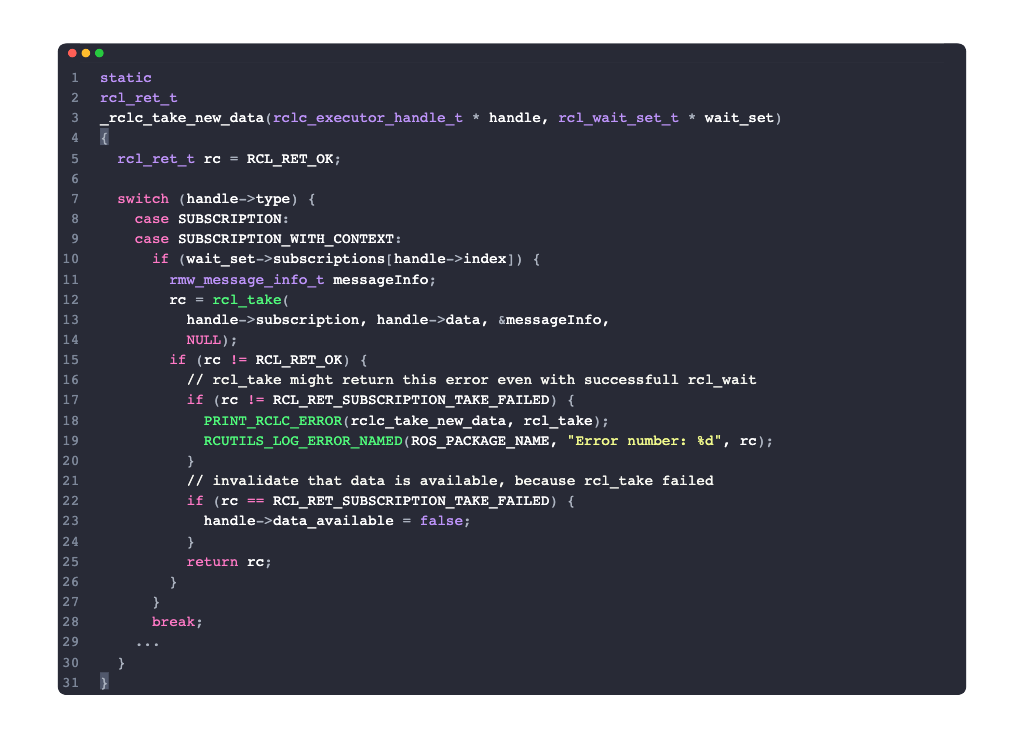
\includegraphics[width=1\linewidth]{Img/code/rclc/_rclc_tak_new_data.png}
    \caption{\_rclc\_let\_scheduling code}
    \vspace{-0.1in}
\end{figure}

% - NOTE:===========================================================================
\subsubsection{\apiarg{\_rclc\_execute}{rclc\_executor\_handle\_t * handle}}
\begin{figure}[htbp!]
    \centering
    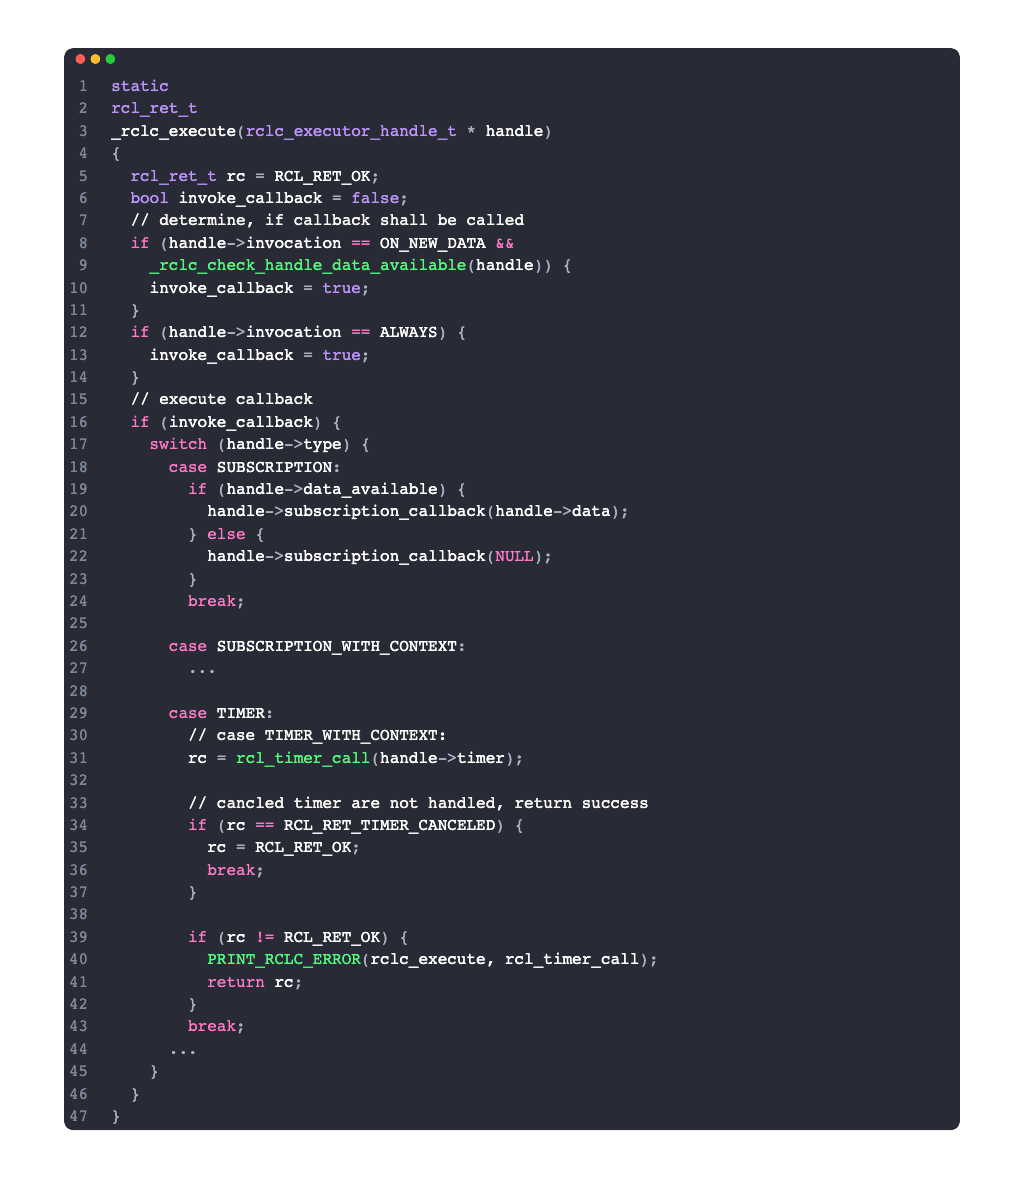
\includegraphics[width=1\linewidth]{Img/code/rclc/_rclc_execute.png}
    \caption{\_rclc\_execute code}
    \vspace{-0.1in}
\end{figure}

\section{RCL}
\subsection{RCL Layer Structures}
% - NOTE: -------------------------------------------------------------
\subsubsection{WORKING: wait.h}
\textbf{1. \str{rcl\_wait\_set\_t}}: 
\begin{figure}[htbp!]
    \centering
    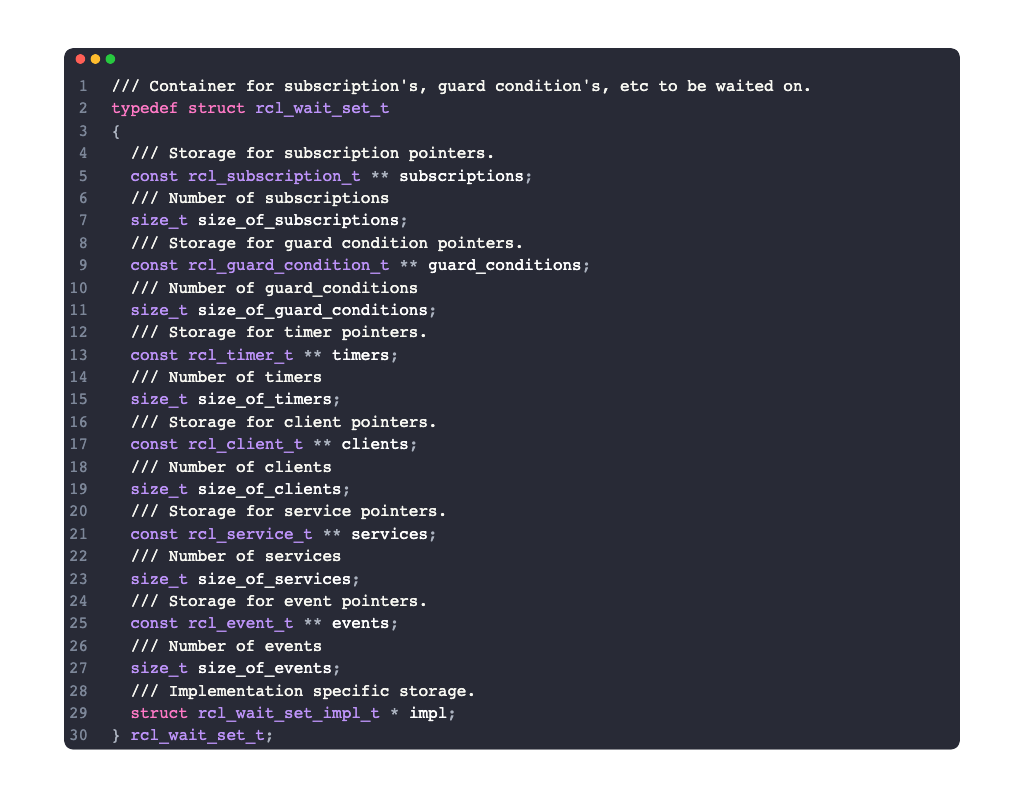
\includegraphics[width=1\linewidth]{Sec/Implementation/rcl/fig/rcl_wait_set_t.png}
    \caption{Structure: rcl\_wait\_set\_t}
    \vspace{-0.1in}
\end{figure}

\textbf{2. \str{rcl\_wait\_set\_impl\_t}}: 
\begin{figure}[htbp!]
    \centering
    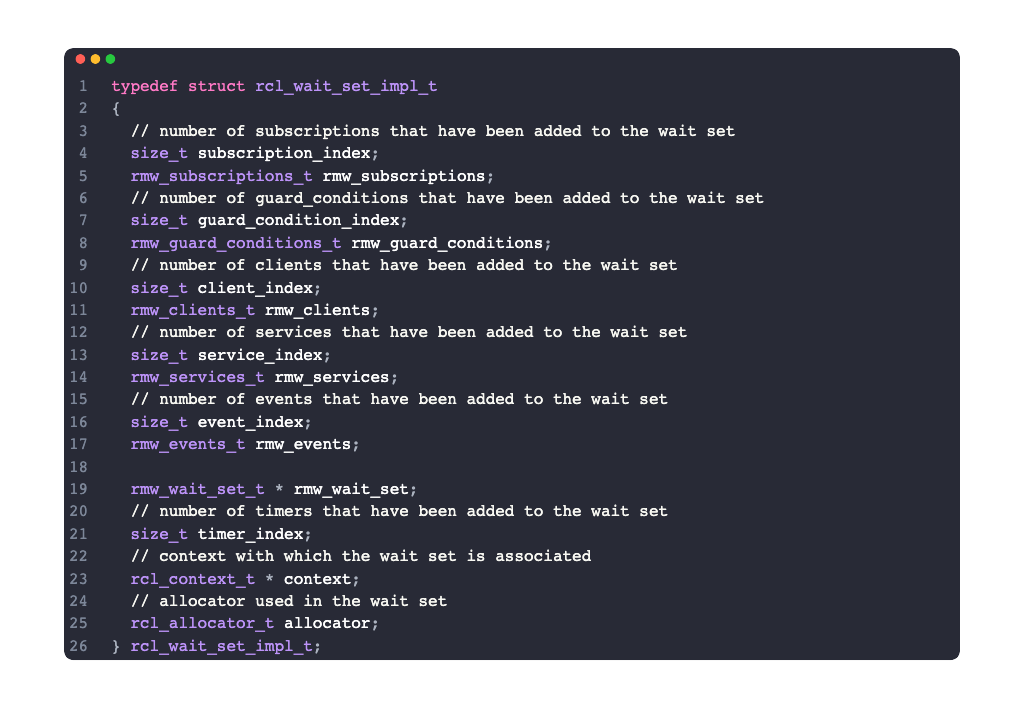
\includegraphics[width=1\linewidth]{Sec/Implementation/rcl/fig/rcl_wait_set_impl_t.png}
    \caption{Structure: rcl\_wait\_set\_impl\_t}
    \vspace{-0.1in}
\end{figure}
\subsection{RCL Layer APIs}
% - NOTE: -------------------------------------------------------------
\subsubsection{WORKING: wait.h}
Wait sets for waiting on messages/service requests and responses/timers to be ready.

\textbf{1. \apiarg{rcl\_wait\_set\_init}{rcl\_wait\_set\_t * wait\_set,
size\_t number\_of\_subscriptions,
size\_t number\_of\_guard\_conditions,
size\_t number\_of\_timers,
size\_t number\_of\_clients,
size\_t number\_of\_services,
size\_t number\_of\_events,
rcl\_context\_t * context,
rcl\_allocator\_t allocator}}: Initialize a rcl wait set with space for items to be waited on. This function allocates space for the subscriptions and other wait-able entities that can be stored in the wait set. It also sets the allocator to the given allocator and initializes the pruned member to be false. The \texttt{wait\_set struct} should be allocated and initialized to \texttt{NULL}. If the \texttt{wait\_set} is allocated but the memory is uninitialized the behavior is undefined. Calling this function on a wait set that has already been initialized will result in an error. A wait set can be reinitialized if \api{rcl\_wait\_set\_fini~()} was called on it.

\textbf{2. \apiarg{rcl\_wait\_set\_add\_subscription}{  rcl\_wait\_set\_t * wait\_set,
const rcl\_subscription\_t * subscription,
size\_t * index}}: Store a pointer to the given subscription in the next empty spot in the set. This function does not guarantee that the subscription is not already in the wait set. Also add the rmw representation to the underlying rmw array and increment the rmw array count.

\textbf{3. \apiarg{rcl\_wait}{rcl\_wait\_set\_t * wait\_set, int64\_t timeout}}: Block until the wait set is ready or until the timeout has been exceeded. This function will collect the items in the \str{rcl\_wait\_set\_t} and pass them to the underlying \api{rmw\_wait~()} function. The items in the wait set will be either left untouched or set to \str{NULL} after this function returns. Items that are not NULL are ready, where ready means different things based on the type of the item. For subscriptions this means there may be messages that can be taken, or perhaps that the state of the subscriptions has changed, in which case \api{rcl\_take~()} may succeed but return with taken == false. For guard conditions this means the guard condition was triggered.








% - NOTE: -------------------------------------------------------------
\subsubsection{WORKING: graph.h}
% - NOTE: -------------------------------------------------------------
\subsubsection{WORKING: init.h}
% - NOTE: -------------------------------------------------------------
\subsubsection{WORKING: guard\_condition.h}
\input{Sec/Implementation/rcl/rcl_static.tex}

\section{RMW}
\subsection{RMW Layer Structures}
% - NOTE: -------------------------------------------------------------
\subsubsection{WORKING: wait}
\textbf{1. \str{rmw\_wait\_set\_t}}: Container for guard conditions to be waited on.
\begin{figure}[htbp!]
    \centering
    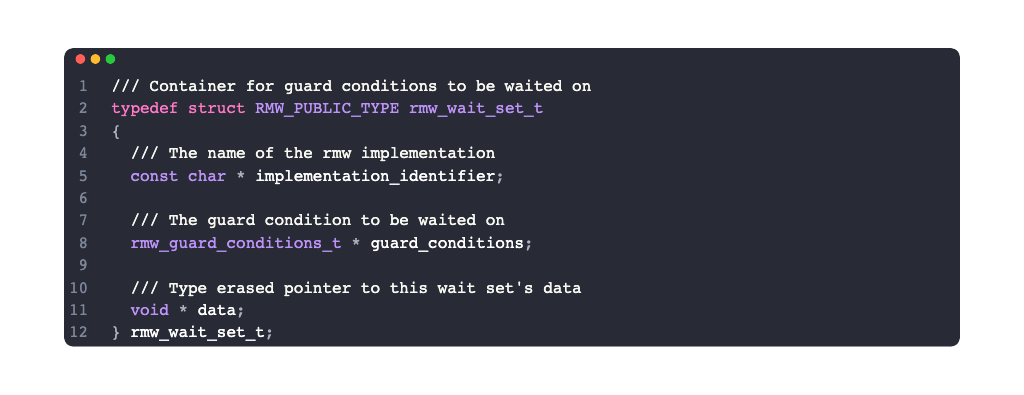
\includegraphics[width=1\linewidth]{Sec/Implementation/rmw/fig/rmw_wait_set_t.png}
    \caption{Structure: rmw\_wait\_set\_t}
    \vspace{-0.1in}
\end{figure}

\textbf{2. \str{rmw\_guard\_conditions\_t}}: Array of guard condition handles. An array of void * pointers representing type-erased middleware-specific guard conditions. The number of non-null entries may be smaller than the allocated size of the array. The number of guard conditions represented may be smaller than the allocated size of the array. The creator of this structure is responsible for allocating and de-allocating the array.
\begin{figure}[htbp!]
    \centering
    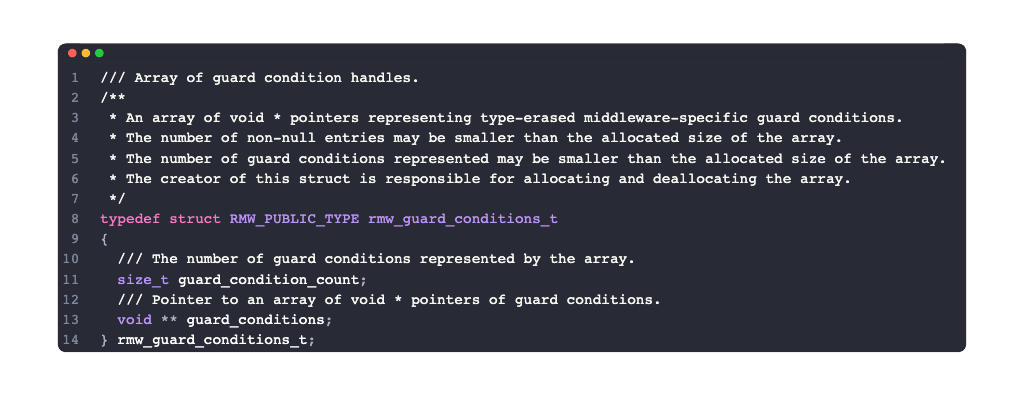
\includegraphics[width=1\linewidth]{Sec/Implementation/rmw/fig/rmw_guard_conditions_t.png}
    \caption{Structure: rmw\_guard\_conditions\_t}
    \vspace{-0.1in}
\end{figure}
\subsection{RMW Layer APIs}
% - NOTE: -------------------------------------------------------------
\subsubsection{INIT: rmw\_init.c}
\todo{HERE!!!!!}


% - NOTE: -------------------------------------------------------------
\subsubsection{WORKING: wait.h}

\textbf{1. \apiarg{rmw\_wait}{  rmw\_subscriptions\_t * subscriptions,
rmw\_guard\_conditions\_t * guard\_conditions,
rmw\_services\_t * services,
rmw\_clients\_t * clients,
rmw\_events\_t * events,
rmw\_wait\_set\_t * wait\_set,
const rmw\_time\_t * wait\_timeout}}: Waits on sets of different entities and returns when one is ready. This function adds middleware-specific conditions to the wait set and waits until one or more become ready, or until the timeout is reached. \footnote{Elapsed time is measured against the system clock. Timeout granularity is thus bound to that of the aforementioned clock and, depending on the underlying implementation, to that of platform-specific APIs to sleep and/or wait. \textbf{The amount of time this function actually waits may be either above or below the specified timeout.}} Called API \api{uxr\_run\_session\_until\_data~()} in XRCE-DDS layer.
\begin{figure}[htbp!]
    \centering
    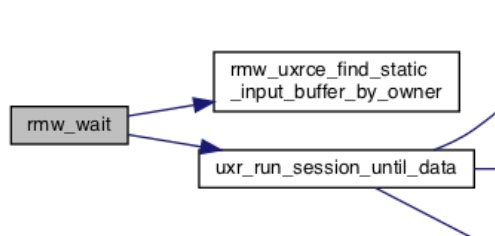
\includegraphics[width=0.5\linewidth]{Sec/Implementation/rmw/fig/rmw_wait().jpg}
    \caption{Function code: rmw\_wait()}
    \vspace{-0.1in}
\end{figure}
\input{Sec/Implementation/rmw/rmw_static.tex}

\section{XRCE-DDS}
\subsection{XRCE-DDS Layer Structures}
% - NOTE: -------------------------------------------------------------
\subsubsection{session.h}
\textbf{1. \str{uxrSession}}: 
\begin{figure}[htbp!]
    \centering
    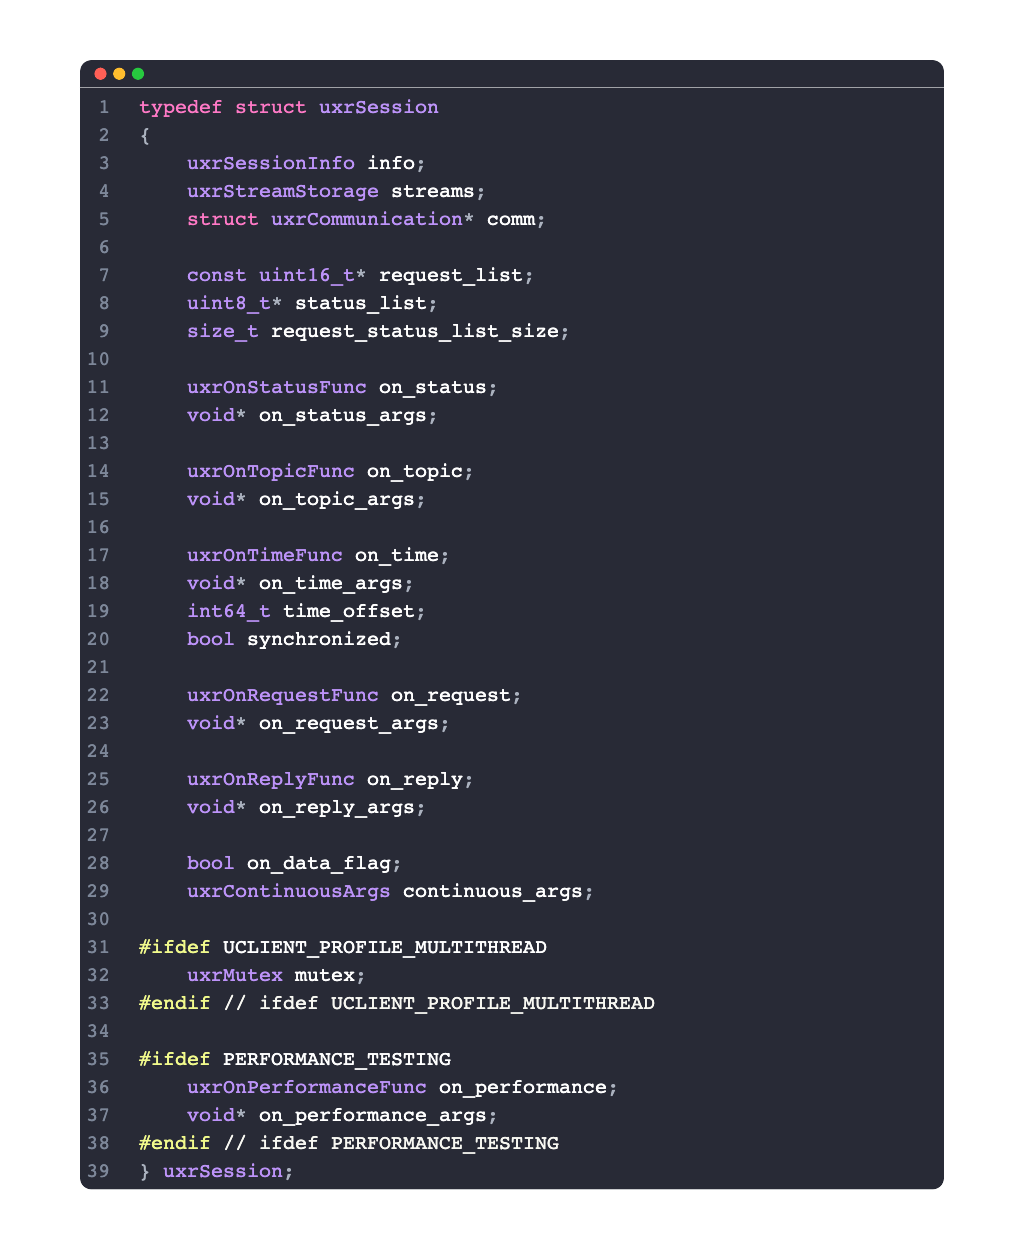
\includegraphics[width=1\linewidth]{Sec/Implementation/uxr/fig/uxrSession.png}
    \caption{Structure: uxrSession}
    \vspace{-0.1in}
\end{figure}


\subsection{XRCE-DDS Layer APIs}
% - NOTE: -------------------------------------------------------------
\subsubsection{session.c}

\textbf{1. \apiarg{uxr\_run\_session\_until\_data}{uxrSession* session, int timeout\_ms}}: Keeps communication between the Client and the Agent. This function involves the following actions:
\begin{itemize}
    \item [(1)] flushing all the output streams sending the data through the transport (e.g., UCP, UART\dots). This actions will be performed in a loop until a data message is received or the \str{timeout} is exceeded.
    \item [(2)] listening messages from the Agent calling the associated callback (topic, status, request and replies).
\end{itemize}

\begin{figure}[htbp!]
    \centering
    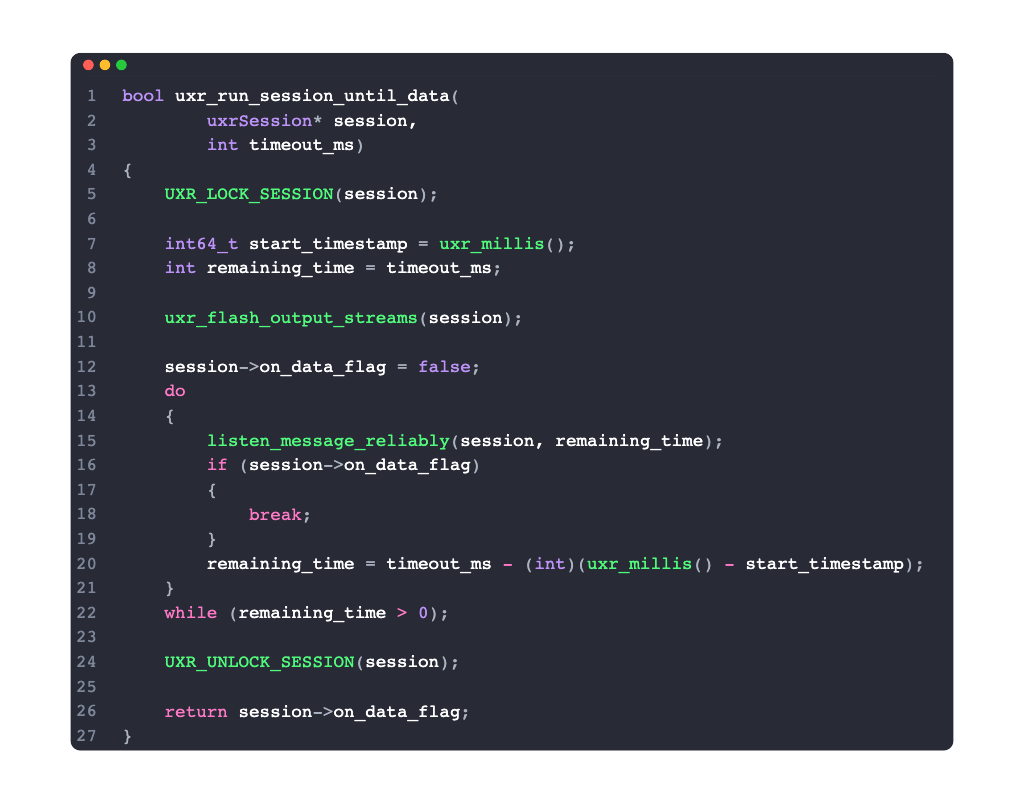
\includegraphics[width=1\linewidth]{Sec/Implementation/uxr/fig/uxr_run_session_until_data.png}
    \caption{Function code: uxr\_run\_session\_until\_data()}
    \vspace{-0.1in}
\end{figure}

As can be seen in function \api{uxr\_run\_session\_until\_data~()}, it first calls \apiarg{UXR\_LOCK\_SESSION}{session}, which finally invokes \apiarg{xSemaphoreTakeRecursive}{mutex->impl, portMAX\_DELAY} on FreeRTOS, or \apiarg{pthread\_mutex\_lock}{\&mutex->impl} on POSIX platform.

\textbf{2. \apiarg{uxr\_stream\_id}{uxrSession* session, int timeout\_ms}}:
\todo{HERE!!!!!!!!!!!!!!!!!!}

\textbf{3. \apiarg{uxr\_prepare\_best\_effort\_buffer\_to\_send}{uxrSession* session, int timeout\_ms}}:

\textbf{4. \apiarg{uxr\_stamp\_session\_header}{uxrSession* session, int timeout\_ms}}:
\input{Sec/Implementation/uxr/uxr_static.tex}

\section{USED POSIX API}

%\input{Sec/2_drt.tex}
%\input{Sec/3_dag.tex}
%\input{Sec/4_scope.tex}
%\input{Sec/5_spinlock}
%\input{Sec/6_conclude}

% \input{Tex/Chap_Guide}
%---------------------------------------------------------------------------%
% main content

% \layout
%-P

%-
%-> Backmatter: bibliography, glossary, index
%-
\backmatter% initialize the environment
\intotoc{\bibname}% add link to contents table and bookmark
% \bibliography{Biblio/ref}% bibliography
\makereference

%
%\chapter{}


\chapter[致谢]{致\quad 谢}\chaptermark{致\quad 谢}% syntax: \chapter[目录]{标题}\chaptermark{页眉}
% \thispagestyle{noheaderstyle}% 如果需要移除当前页的页眉
%\pagestyle{noheaderstyle}% 如果需要移除整章的页眉

\reviewORprint{
}{

六年的博士生活即将结束,在这里我由衷地感谢多年来给予我无私帮助和关怀的老师、同学、朋友和家人。

首先要感谢我的导师王义教授。是您让我有机会来到智慧系统实验室这个大集体,是您引领我进入了科研的大门。感谢您在我的学习生涯中提供的宝贵支持、指导和建议。王老师严谨的治学态度让我受用一生,做学问一定要踏实认真,精益求精,不要一味追求出成果,要懂得过程的重要性。同时,您工作和生活中充沛的精力同样感染着我,教会了我永不放弃,保持一颗积极乐观的态度去面对多彩的学习和生活。您的治学风格和人格魅力使我受益终生。在此向我的导师王义教授表示衷心的感谢与祝福!

感谢关楠教授。在您身边受教已近五载,您不但提供给我高水平的研究平台,还对我的工作进行了大量具体的指导。您的诸多教诲,诸如“换个角度看问题”,“只要肯思考,办法总比困难多”,“不要逃避问题”等等让我受益匪浅。在未来的工作中,我会以您为榜样,谨记您的教诲,知行合一,自强不息!

感谢吕鸣松教授。您不但在工作和生活上给予我大量的帮助,更在为人处世上传授我诸多经验,使我的性格更加成熟。您认真严谨的学术态度是我学习的榜样,在此向吕老师表达我最诚挚的感谢!

感谢其他各位老师、同学和朋友的关心与帮助。能够生活和学习在这样温馨的大集体中,是我人生难忘的经历。感谢魏阳杰教授在我攻读博士期间对我的关心和照顾,您的谦逊和乐观是我学习的榜样。感谢东北大学智慧系统实验室的同学王样,唐月,纪东等等,能够和你们一起成长使我倍感幸运。感谢访问香港理工大学期间的同学姜徐,何青强等,你们的聪明才智给我的研究工作带来了取之不尽的灵感。特别感谢张伟同学,在我学术遇到困难时给予的支撑与帮助。特别感谢刘卓然同学,相识十载我们一起度过了愉快的大学及博士时光,感谢你在我学习生活遇到困难时给予的支持和鼓励。感谢刘松冉同学,多年来在工作、学习和生活方面对我的帮助,我很幸运能遇到你这样的好师兄。还有诸多好友,篇幅所限无法一一列举诸位名姓,感谢你们的每一次帮助!

感谢我的父母。你们无私的爱与包容,是我坚强的后盾和前行的动力。你们的恩情我穷尽一生也无法报答,我定当竭力进取以求不负你们之厚望。并祝愿我的亲人们身体健康,喜乐长安。

还要感谢我的爱人陶力辉。在我学术生活遇到困难时,给予理解与安慰。感谢你的体谅与包容,这本薄薄的论文是献给你的礼物。

最后要感谢评阅本论文的各位老师及朋友,谢谢你们抽出了宝贵的时间并给予我中肯的建议。

}

\chapter{攻读博士学位期间取得的学术成果}


\reviewORprint{
    \section*{第一作者发表/录用学术论文:}
    \begin{enumerate}[leftmargin=*]
        \item Title[J]Journal, Year, Volume(Number):Pages. (\textbf{SCI, JCR1, 论文第三章})
    \end{enumerate}
    \section*{第一作者在审学术论文:}
    \begin{enumerate}[leftmargin=*]
        \item Title[J]Journal, Year, Volume(Number):Pages. (\textbf{SCI, JCR1, 论文第三章})
    \end{enumerate}
    \section*{通讯作者发表/录用学术论文:}
    \begin{enumerate}[leftmargin=*]
        \item Title[J]Journal, Year, Volume(Number):Pages. (\textbf{SCI, JCR1, 第二作者/通讯作者})
    \end{enumerate}
    \section*{合作作者发表/录用学术论文:}
    \begin{enumerate}[leftmargin=*]
        \item Title[J]Journal, Year, Volume(Number):Pages. (\textbf{SCI, JCR1, 第二作者})
    \end{enumerate}
}{
    \section*{学术论文:}
    \begin{enumerate}[leftmargin=*]
        \item \textbf{He Du}, Wei Zhang, Nan Guan, Wang Yi. Scope-aware data cache analysis for OpenMP programs on multi-core processors[J]. Journal of Systems Architecture, 2019, Volume(98): 443--452. (SCI检索, CCF-B, 论文第四章)
        \item \textbf{He Du}, Xu Jiang, Tao Yang, Mingsong Lv, Wang Yi. Real-Time Scheduling and Analysis of OpenMP Programs with Spin Locks[C]. IEEE International Conference on Parallel and Distributed Systems (ICPADS), Hong Kong, 2-4 December, 2020. (EI, CCF-C, 论文第五章)
        \item \textbf{He Du}, Xu Jiang, Mingsong Lv, Tao Yang, Wang Yi. Scheduling and Analysis of Real-Time Task Graph Models with Nested Locks[J]. Journal of Systems Architecture, Volume 114, March 2021, 101969. (SCI, CCF-B, 论文第二章)
        \item Xu Jiang, Nan Guan, \textbf{He Du},  Weichen Liu, Wang Yi. On the Analysis of Parallel Real-Time Tasks with Spin Locks[J]. 2020 IEEE Transactions on Computers, Volume(67): 975--991. (SCI, CCF-A, 论文第三章)

    \end{enumerate}
}

\section*{科研项目:}

\begin{enumerate}[leftmargin=*]
    \item 国家自然科学基金重点项目:混合关键型多核嵌入式软件设计、验证与优化关键技术研究(67532007),2016年1月至2020年12月,主要参与者。
    \item 国家自然科学基金重点项目:面向GPU的实时系统时间分析与优化技术研究(61772123),2018年1月至2021年12月,主要参与者。
\end{enumerate}

\forget{

\chapter{个人简历}
杜贺,女,汉族,1993年6月出生于辽宁省沈阳市。2011年考入东北大学信息科学与工程学院计算机专业,于2015年7月毕业,获得工学学士学位。同年保送本校博士研究生,师从王义教授和关楠教授。主要从事实时系统中实时调度算法及并行程序分析的研究工作。2017年至今访问香港理工大学,师从关楠教授。

2015年至今,致力于系统中实时调度算法设计、共享资源的实时锁协议设计与并行程序分析等研究。攻读博士学位期间,共发表论文4篇,其中第一作者被SCI收录2篇,第一作者被EI收录1篇。研究成果发表在ICPADS、JSA等国际著名会议和期刊中。
%作为项目主要参与人己完成和正在参与的科研项目主要有国家自然科学基金:混合关键系统动态实时调度与容错设计研究(67532007),面向GPU的实时系统时间分析与优化技术研究(61772123)等。

}

\cleardoublepage[plain]% 让文档总是结束于偶数页,可根据需要设定页眉页脚样式,如 [noheaderstyle]

% other information
% \showthe\artxfontset
\end{document}
%---------------------------------------------------------------------------%

